\documentclass{article}
\usepackage[linesnumbered,ruled,longend]{algorithm2e}
\usepackage{amsmath, amssymb, amsthm}
\usepackage{multicol, relsize, geometry}
\usepackage{booktabs}
\usepackage{hyperref}
\usepackage{graphicx}
\usepackage{pgfplots}
\usepackage{pgfplotstable}
\usepackage{caption}
\usepackage{pgfplotstable}
\usepackage{indentfirst}
\usepackage{setspace}
\usepackage[none]{hyphenat}

\singlespacing
% Adjust spacing between paragraphs
\setlength{\parskip}{1ex plus 0.5ex minus 0.2ex}
\setlength\parindent{24pt}

% Add packages for font and encoding
\usepackage[T1]{fontenc}
\usepackage[utf8]{inputenc}
\usepackage{mathptmx} % Times New Roman font

% Set font size and line spacing
\usepackage{setspace}
\fontsize{10}{12}\selectfont % 10pt font size with 12pt leading
\singlespacing % Ensure single spacing within paragraphs
% Needs to be last
\usepackage[table]{xcolor}

\DontPrintSemicolon
\SetKwFor{For}{for}{do}{end for}
\SetKwIF{If}{ElseIf}{Else}{if}{then}{else if}{else}{end if}%
% Redefine \ForEach to display a vertical line under it
\SetKwFor{ForEach}{for each}{}{end for}
\geometry{top=1cm, bottom=2cm, left=1cm, right=1cm}
\newcommand{\pluseq}{\mathrel{+}=}
\title{A heterogeneous vehicle routing problem with drones and multiple depots}
\author{Panagiotis Zachos}
\date{June 2024}

\begin{document}
	\maketitle
	
	\section{Multi-Depot mixed fleet capacitated multiple TSP}
	The problem takes as input a set of nodes, comprising of customer nodes and depot nodes. Each depot may be equipped with a heterogeneous fleet of vehicles: Trucks, Motorbikes, and Drones. Each vehicle type has a specific capacity k, representing the number of parcels it can carry. The vehicles initiate their routes from their respective depots, fully loaded with parcels, and visit customer nodes, each with a demand of one parcel. Upon completing a route, either due to no customers remaining or reaching capacity,  the vehicle returns to its depot, where it is reloaded to full capacity and can be dispatched again if there are remaining customers. The aim is to visit all customers in the minimum possible time, with \textbf{no restriction on the total number of parcels available at each depot}, thus differing from traditional MDVRP constraints.
	\par
	\begin{figure}[h]
		\caption{Solution example}
		\centering
		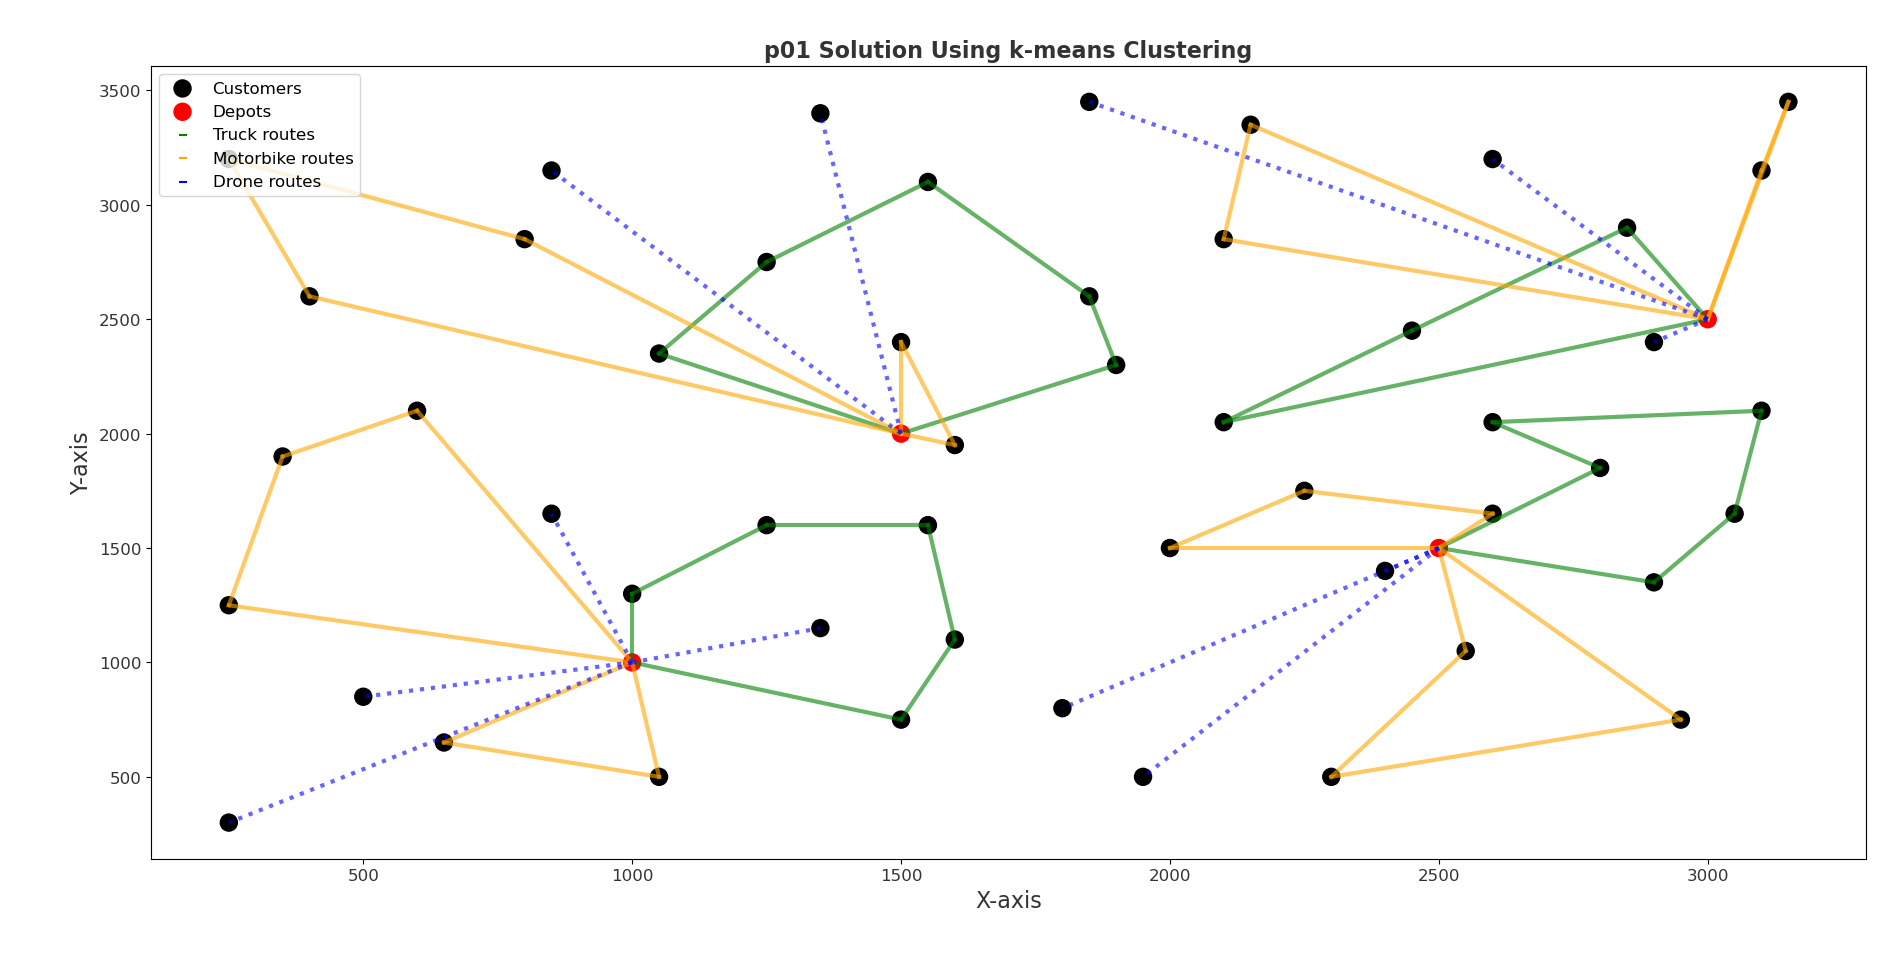
\includegraphics[width=\textwidth]{Solution-example}
	\end{figure}
	\twocolumn
	\subsection{Objective}
	The objective of the MD-mfcmTSP is to minimize the total makespan in which all customers have been served i.e min $M_{total}$.\;
	\newline
	\newline
	\textbf{Notation}\;
	\begin{itemize}
		\item $m$ : Number of depots
		\item $D$ : Set of depots
		\item $R_T^i$ : Truck route of depot $i\in D$ \;
		\item $R_M^i$ : Motorbike route of depot $i\in D$ \;
		\item $R_D^i$ : Drone route of depot $i\in D$ \;
		\item $M_T^i$ : Makespan of Truck route of depot $i\in D$ \;
		\item $M_M^i$ : Makespan of Motorbike route of depot $i\in D$ \;
		\item $M_D^i$ : Makespan of Drone route of depot $i\in D$ \;
		\item $M_T$ = $max(M_T^i, M_T^{i+1}, ..., M_T^m)$ : Makespan of Trucks \;
		\item $M_M$ = $max(M_M^i, M_M^{i+1}, ..., M_M^m)$ : Makespan of Motorbikes \;
		\item $M_D$ = $max(M_D^i, M_D^{i+1}, ..., M_D^m)$ : Makespan of Drones \;
		\item $M_{total}$ = $max(M_T, M_M, M_D)$ : Total makespan \;
	\end{itemize}
	\begin{table}[h!]
	\centering
	\caption{Example}
	\resizebox{0.3\columnwidth}{!}{%
		\begin{tabular}{@{}ccccc@{}}
			\toprule
			\textbf{Depot} & \textbf{$M_T$} & \textbf{$M_M$} & \textbf{$M_D$} & \textbf{Depot makespan} \\ 
			\midrule
			1 & 3 & 2 & 1 & 3 \\
			\midrule 
			2 & 4 & 3 & 2 & 4 \\
			\midrule 
			3 & 1 & 5 & 2 & 5 \\
			\midrule 
			4 & 2 & 8 & 1 & 8 \\
			\midrule
			\textbf{$M_{total}$} & 4 & \textbf{8} & 2 & \textbf{8} \\
			\bottomrule
		\end{tabular}%
	}
\end{table}
	\twocolumn
	\section{Makespan calculations}
	In the case where a depot is equipped with more than 1 vehicle of either type, the makespan calculations are explained below.
	Assume 4 routes that need to be assigned to two trucks. Each route has a time cost associated with it. The route assignment needs to be done in such a way that the trucks' makespan is minimized. We first sort the routes based on their cost in a descending order. Then, starting from the route with the maximum cost, we assign it to the truck with the currently minimum makespan. This is done iteratively until all routes have been assigned to a vehicle. 
	\begin{table}[h!]
	\centering
	\caption{4 routes that need to be assigned to a depot's 2 trucks}
	\resizebox{0.12\columnwidth}{!}{%
		\begin{tabular}{@{}cc@{}}
			\toprule
			\textbf{Route} & \textbf{Cost} \\ 
			\midrule
			1 & 5 \\
			\midrule 
			2 & 6 \\
			\midrule 
			3 & 2 \\
			\midrule 
			4 & 3 \\
			\bottomrule
		\end{tabular}%
	}
\end{table}
\newline
\textbf{Procedure for the assignment of 4 routes to 2 trucks of the same depot:}
\begin{table}[h!]
	\centering
	\caption{Sort routes in descending order based on cost}
	\resizebox{0.12\columnwidth}{!}{%
		\begin{tabular}{@{}cc@{}}
			\toprule
			\textbf{Route} & \textbf{Cost} \\ 
			\midrule
			2 & 6 \\
			\midrule 
			1 & 5 \\
			\midrule 
			4 & 3 \\
			\midrule 
			3 & 2 \\
			\bottomrule
		\end{tabular}%
	}
\end{table}
\begin{table}[h!]
	\centering
	\caption{Iteratively assign routes to Trucks}
	\resizebox{0.5\columnwidth}{!}{%
		\begin{tabular}{@{}cccccc@{}}
			\toprule
			\textbf{Iteration} & \textbf{Route} & \textbf{Cost} & \textbf{Truck} & \textbf{Truck 1 ms} & \textbf{Truck 2 ms}\\ 
			\midrule
			1 & 2 & 6 & 1 & 6 & 0\\
			\midrule 
			2 & 1 & 5 & 2 & 6 & 5\\
			\midrule 
			3 & 4 & 3 & 2 & 6 & 8\\
			\midrule 
			4 & 3 & 2 & 1 & 8 & 8\\
			\midrule
			\multicolumn{6}{@{}c@{}}{Total makespan = 8 (optimal)}\\
			\bottomrule
		\end{tabular}%
	}
\end{table}
	
	\onecolumn
	\clearpage
	\subsection{Motivation / Use case}
	By introducing this problem, we contribute to the Travelling Salesman Problem and Vehicle Routing Problem research and the field of logistics and routing by introducing a realistic and challenging problem that considers the practical limitations and requirements of different vehicle types used in last-mile delivery. The proposed algorithms have the potential to improve efficiency and reduce costs for logistics companies operating in increasingly complex delivery environments.
	\par 
	Consider a parcel delivery company operating in Greece, with depots located in two major cities: Athens and Thessaloniki. The company manages numerous last-mile delivery shops in these cities, which serve as depots in the routing problem. For instance, a customer in Thessaloniki sends a parcel to a friend in Athens by visiting a nearby shop. After the shop stops receiving parcels for the day, a truck collects the parcels and delivers them to the Thessaloniki distribution center. Parcels destined for Athens are then transported overnight to the Athens distribution center.
	Upon arrival, parcels are sorted based on their delivery areas and sent to the appropriate last-mile shops in Athens. These shops, acting as depots in our problem, dispatch vehicles (Trucks, Motorbikes, Drones) to deliver the parcels to their final destinations. The MD-mfcmTSP addresses how these vehicles can be optimally routed to minimize delivery time, while simultaneously solving the problem of parcel allocation in each last-mile shop.
	\par
	\begin{figure}[h!]
		\caption{Life of a parcel}
		\centering
		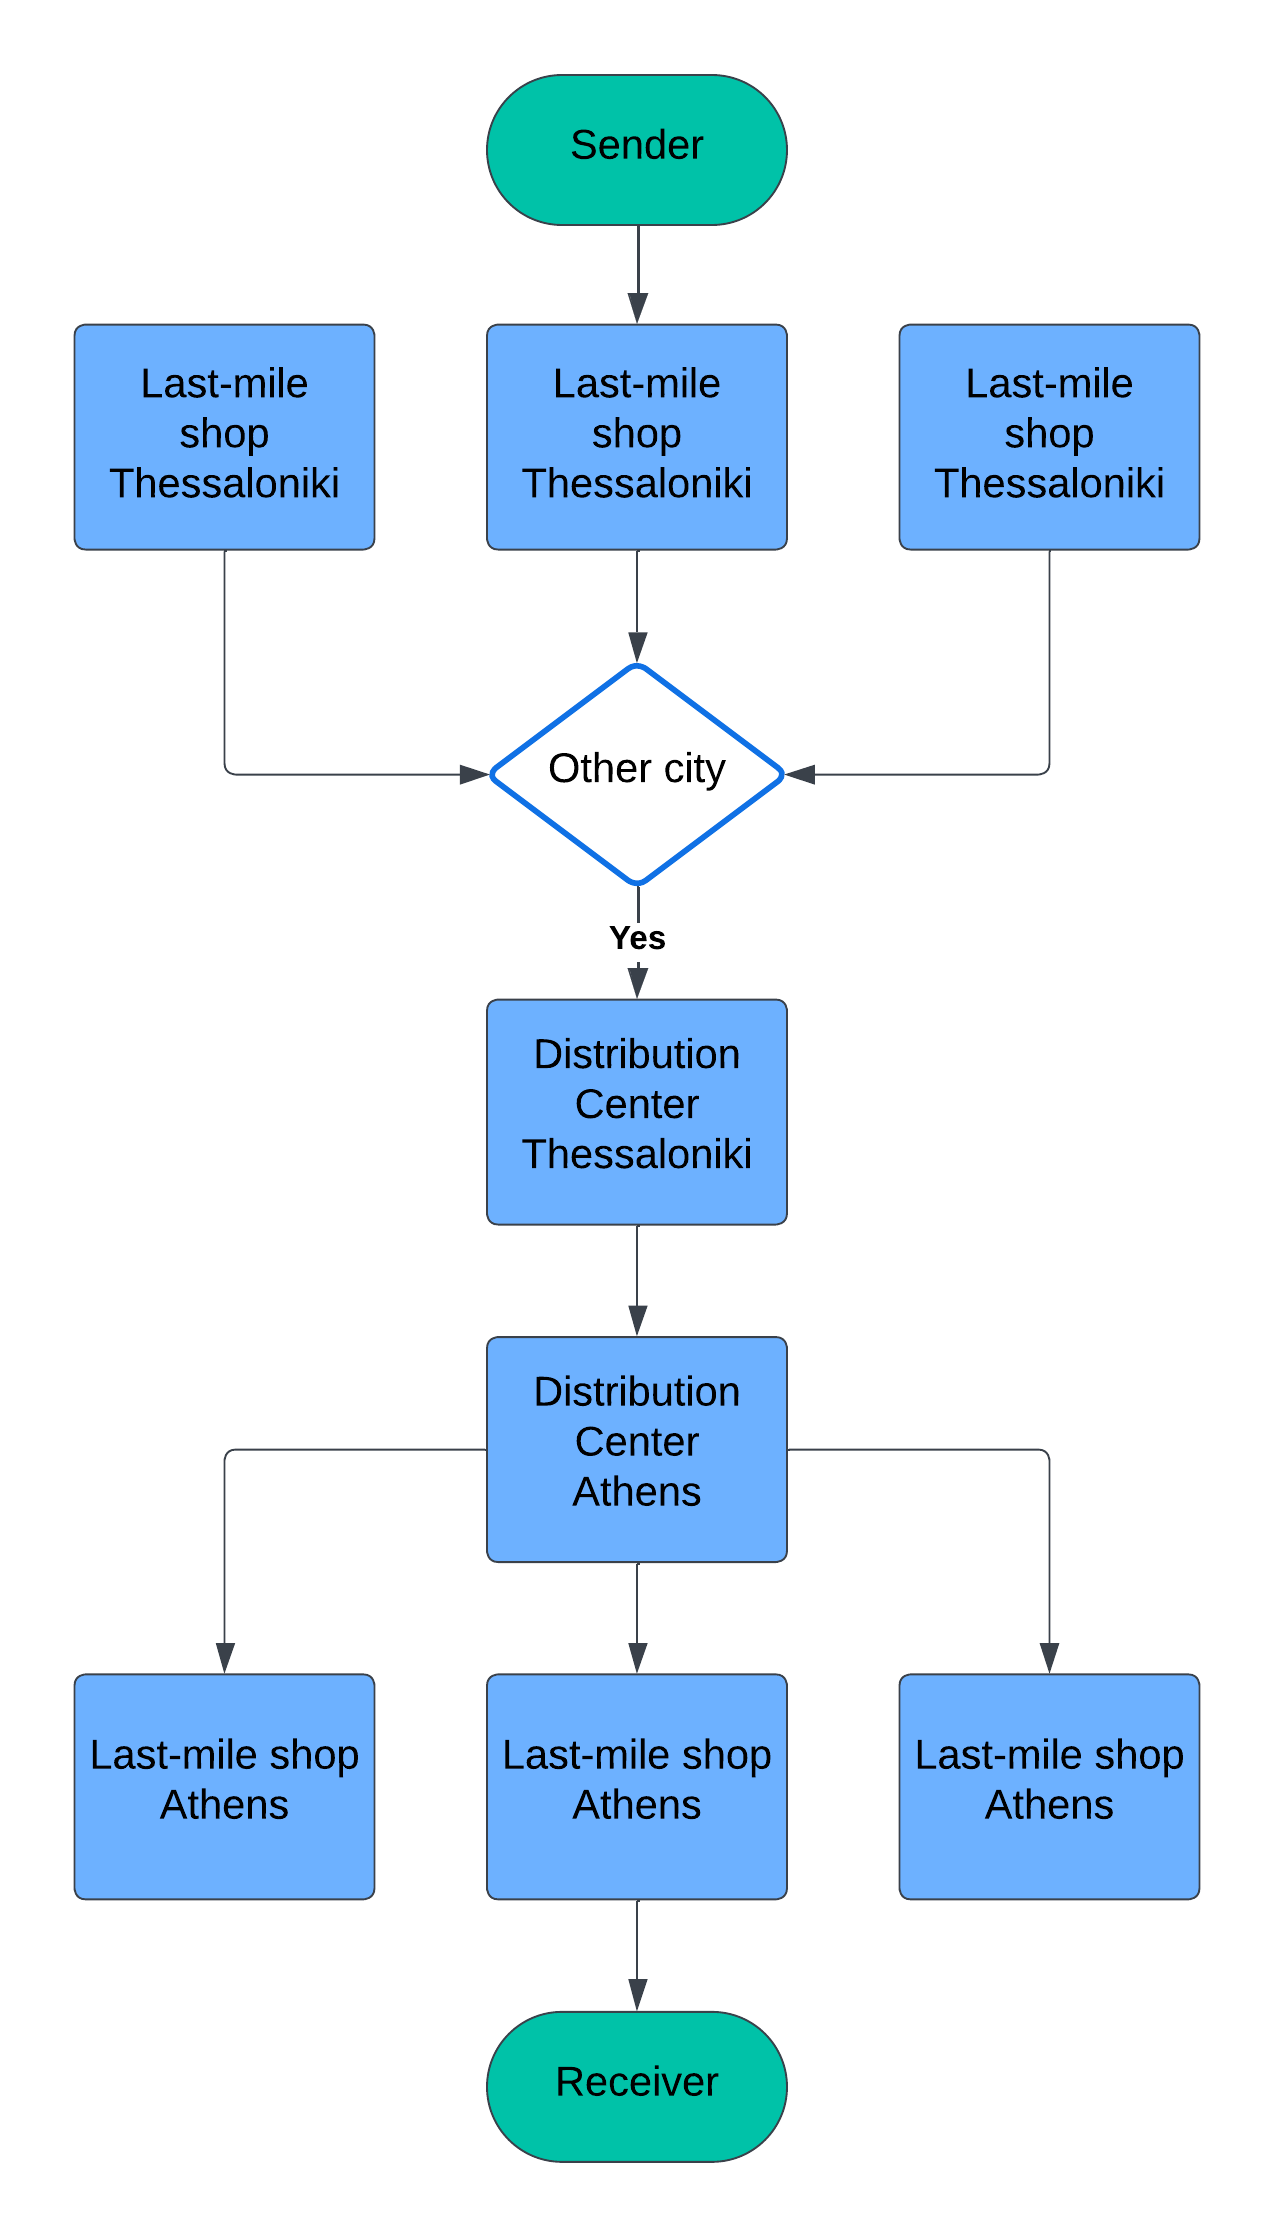
\includegraphics[width=0.40\textwidth, height=0.50\textheight]{Parcel-Life}
	\end{figure}
	\clearpage
	\twocolumn
	\section{Problem description}
	\begin{itemize}
		\item Each customer must be visited exactly once
		\item Each vehicle can serve at most as many customers per trip as its capacity
		\item Some customers may not be available for delivery via uav or larger vehicles
		\item Each depot must be equipped with at least one truck
		\item The composition of each depot's fleet is known
		\item Depots act as a start, finish and reload point for their fleet
		\item Each vehicle may perform unlimited routes (multi-trip)
	\end{itemize}
	
	\section{Pseudocode for the MD-mfcmTSP}
	At the end of Algorithm 1, a local optimization function (3) is called which in addition to moving nodes in different places in the same route, also moves nodes between routes of different depots and different vehicle types.\;
	\begin{algorithm}
		\small
		\caption{MD-mfcmTSP heuristic}
		\label{alg:MDmfcmTSP}
		\KwIn{$G_T, G_M, ..., G_D$}
		\KwOut{$M_{total}$, $Sol = \{Sol^i = \{R_T^i, R_M^i, ...,R_D^i\}, Sol^{i+1}, ..., Sol^m\}$ for each $i\in D$}
		
		Create clusters $K^i$ of customer nodes for each depot $d^i\in D$\;
		by assigning each customer to the closest possible depot\;
		\For{each $d^i\in D$}{
			
			Call $Initialization(d^i, K^i)$\;
			\While{$(M_T^i > M_M^i\parallel M_T^i > M_D^i)$ $\&\&$ $stop\neq true$}{
				$diff_M = M_T^i - M_M^i$\;
				$diff_D = M_T^i - M_D^i$\;
				\uIf{$diff_M\ge diff_D$}{
					$vt = M$\;
					$cap =$ Motorbike's capacity\;
				}\Else{
					$vt = D$\;
					$cap =$ 1\;
				}
				$M_{min} = M_T^i$\;
				$r_{best} = \emptyset$\;
				\For{$j=1$ to $|R_T^i| - cap$}{
					$successive\_nodes = \emptyset$\;
					$load = 0$\;
					\While{$load + v_j^{demand} \leq cap$ $\&\&$ $v_j\in G_{vt}$}{
						$successive\_nodes \pluseq v_j$\;
					}
					\If{$|successive\_nodes| == cap$}{
						$r_{new} = R_T^i[0] + \{successive\_nodes\} + R_T^i[0]$\;
						${R'}_{vt}^i = R_{vt}^i + r_{new}$\;
						${M'}_{vt} = {R'}_{vt}^i$ 's makespan\;
						${R'}_T^i = R_T^i - \{successive\_nodes\}$\;
						${M'}_T = {R'}_T^i$ 's makespan\;
						$M_{new} = MAX({M'}_T, {M'}_{vt})$\;
						\If{$M_{new} < M_{min}$}{
							$M_{min} = M_{new}$\;
							$r_{best} = r_{new}$\;
						}
						$r_{new} = \emptyset$\;
					}
					$j\pluseq 1$\;
				}
				\uIf{$r_{best} \neq \emptyset$}{
					$R_T^i = R_T^i - \{r_{best}^{customers}\}$\;
					$M_T = R_T^i$ 's makespan\;
					$R_{vt}^i\pluseq r_{best}$\;
					$M_{vt} = R_{vt}^i$ 's makespan\;
					Call $local\_optimization(R_T^i, n_{max})$\;
					Call $local\_optimization(R_{vt}^i, n_{max})$\;
				}\Else{ 
					$stop = true$\;
				}
			}
			$Sol^i = \{R_T^i, R_M^i, ..., R_D^i\}$\;
		}
		$M_T = MAX(M_T^i, M_T^{i+1}, ..., M_T^m)$\;
		$M_M = MAX(M_M^i, M_M^{i+1}, ..., M_M^m)$\;
		$M_D = MAX(M_D^i, M_D^{i+1}, ..., M_D^m)$\;
		$M_{total} = MAX(M_T, M_M, ..., M_D)$\;
		Call $optimization\_full(Sol, n_{max})$
	\end{algorithm}
	
	\begin{algorithm}
		\small
		\caption{Initialization($d^i, K^i$)}
		\label{alg:initialization}
		\While{$\{K^i\}\cap \{G_T\}\neq \emptyset$}{
			$R_T^i\pluseq NearestNeighbour(\{K^i\}\cap \{G_T\})$\;
		}
		$M_T^i = R_T^i$ 's makespan\;
		$v_{free} = \{K^i\} - \{G_T\}$\;
		\uIf{$v_{free} = \emptyset$}{
			\Return{$R_T^i$}\;
		}\Else{
			\While{$v_{free}\neq \emptyset$}{
				\uIf{$M_T - M_M\geq M_T - M_D \parallel G_D = \emptyset$}{
					$R_M^i\pluseq NearestNeighbour(\{K^i\}\cap \{G_M\})$\;
					$v_{free} = v_{free} - \{R_M^i\}$\;
					$M_M^i = R_M^i$ 's makespan\;
				}\Else{
					$R_D^i\pluseq closest(\{K^i\}\cap \{G_D\})$\;
					$M_D^i = R_D^i$ 's makespan\;
				}
			}
		}
		\Return{$Sol^i$}\;
	\end{algorithm}
	
	\begin{algorithm}
		\small
		\caption{$optimization\_full(Sol, n_{max})$}
		Call $vt\_optimization(Sol, n_{max} = 2)$\;
		\For{each $vt$}{
			\For{each $i\in D$}{
				Call $local\_optimization(R_{vt}^i, n_{max}=2)$\;
			}
			Call $mutual\_depot\_optimization(R_{vt}, n_{max}=2)$\;
		}
		Call $vt\_optimization(Sol, n_{max} = 2)$\;
	\end{algorithm}
	
	\begin{algorithm}
		\small
		\caption{$local\_optimization(r, n_{max})$}
		\For{$n=1$ to $n_{max}$}{
			\ForEach{combination of $n$ successive nodes on the route}{
				move the node(s) to a different place on the same route\;
				evaluate the new route\;
				\uIf{this route is better than the original and all constraints are satisfied}{
					replace the original route with the new one\;
				}
				continue in point 3 unless all possible places in the route have been evaluated\;
			}
		}
		\Return{$r$}\;
	\end{algorithm}
	
	\begin{algorithm}
		\small
		\caption{$mutual\_depot\_optimization(R_{vt}, n_{max})$}
		\For{$n = 1$ to $n_{max}$}{
			\ForEach{possible pair of depots $c1$ and $c2$}{
				\ForEach{combination of $n$ successive nodes in the route of c1}{
					remove the nodes from the route of c1 and insert them into c2\;
					evaluate the newly-created routes\;
					\uIf{$MAX(|{R'}_{vt}^{c1}|, |{R'}_{vt}^{c2}|) < MAX(|{R}_{vt}^{c1}|, |{R}_{vt}^{c2}|)$ and all constraints are satisfied}{
						replace the original routes with the new ones\;
					}
					continue in point 4 unless all possible places in c2 have been evaluated\;
				}
			}
		}
		\Return{$R_{VT}$}\;
	\end{algorithm}
	
	\begin{algorithm}
		\small
		\caption{$vt\_optimization(Sol, n_{max})$}
		\For{$n = 1$ to $n_{max}$}{
			\ForEach{depot $i\in D$}{
				\ForEach{possible pair of vehicle types $t1,t2\in VT$}{
					\ForEach{combination of $n$ successive nodes in $R_{t1}^i$}{
						remove the nodes from $R_{t1}^i$ and insert them in $R_{t2}^i$\;
						\uIf{$MAX(|{R'}_{t1}^i|, |{R'}_{t2}^i|) < MAX(|{R}_{t1}^i|, |{R}_{t2}^i|)$ and all constraints are satisfied}{
							replace the original routes with the new ones\;
						}
						continue in point 5 unless all possible places in $R_{t2}^i$ have been evaluated\;
					}
				}
			}
		}
		\Return{$Sol$}\;
	\end{algorithm}
	\clearpage
	\begin{figure*}[h]
		\caption[width=\textwidth]{p11 Initialization example using k-means clustering}
		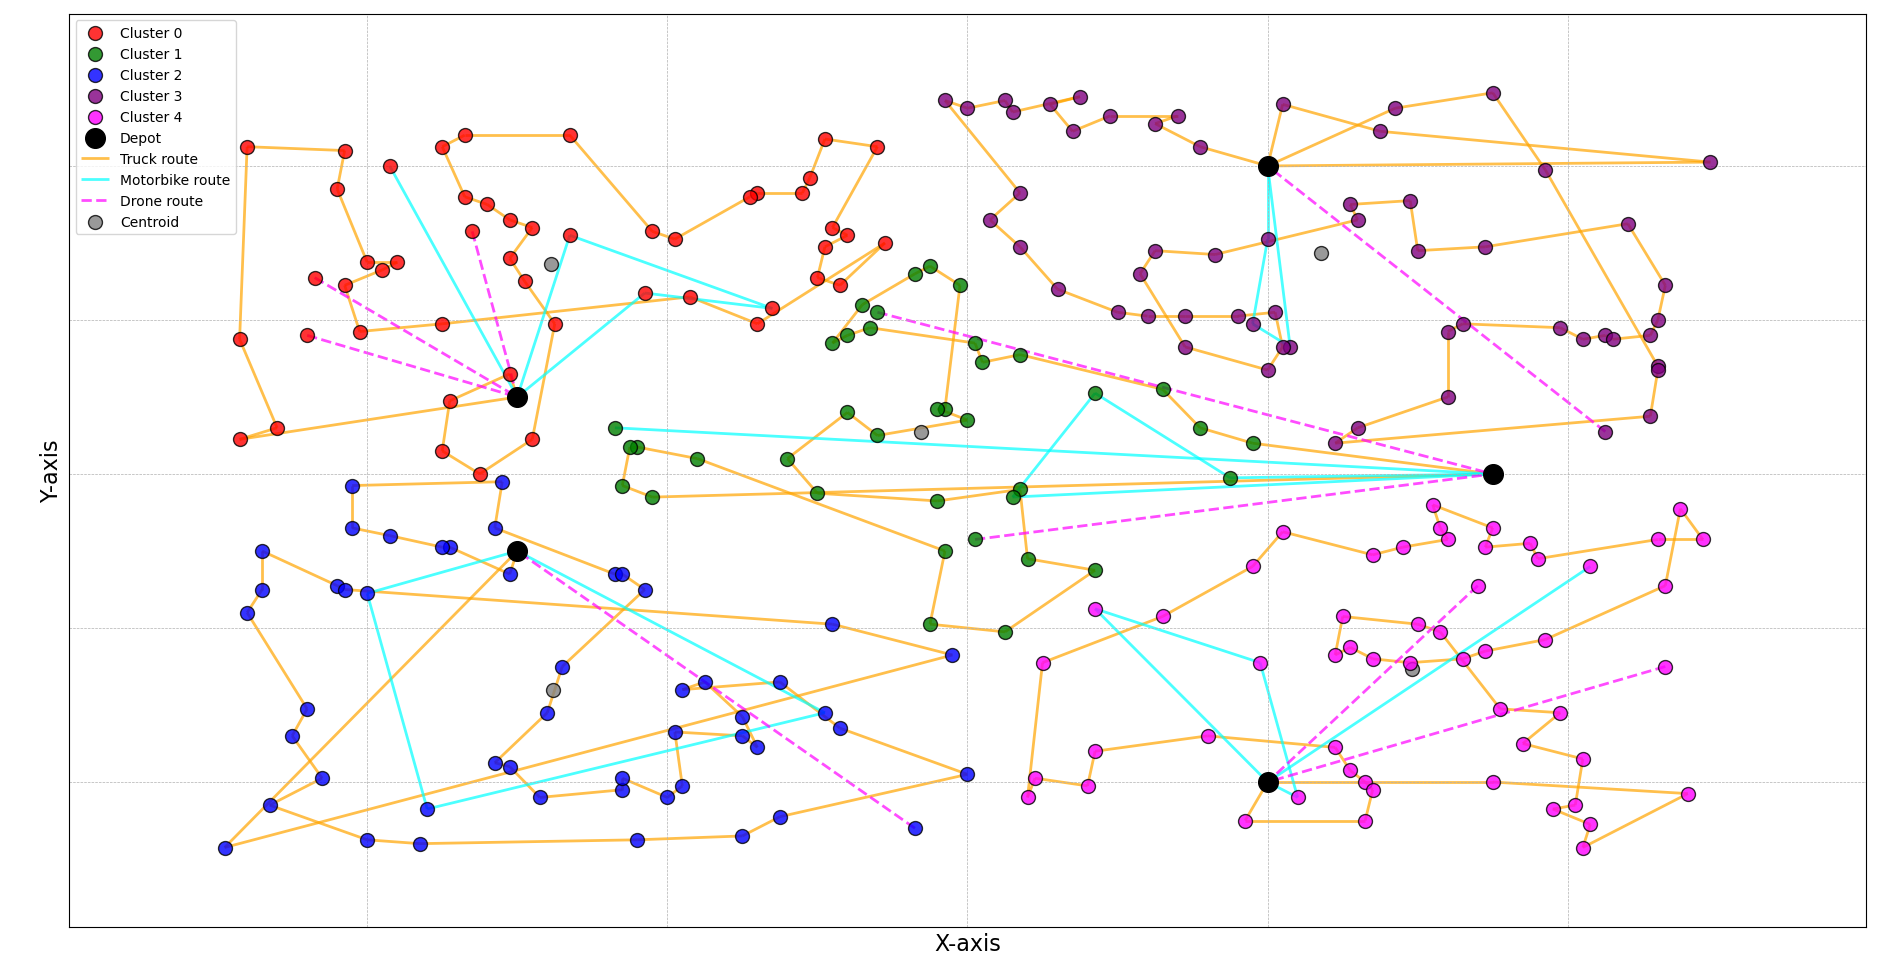
\includegraphics[width=\textwidth]{Initialization_example_p11}
		\centering
	\end{figure*}
	\begin{figure*}[h]
		\caption[width=\textwidth]{p01 initialization using k-means clustering}
		\includegraphics[width=\textwidth]{initialization_example_p01}
		\centering
	\end{figure*}
	\begin{figure*}[h]
		\caption[width=\textwidth]{p01 solution using k-means clustering}
		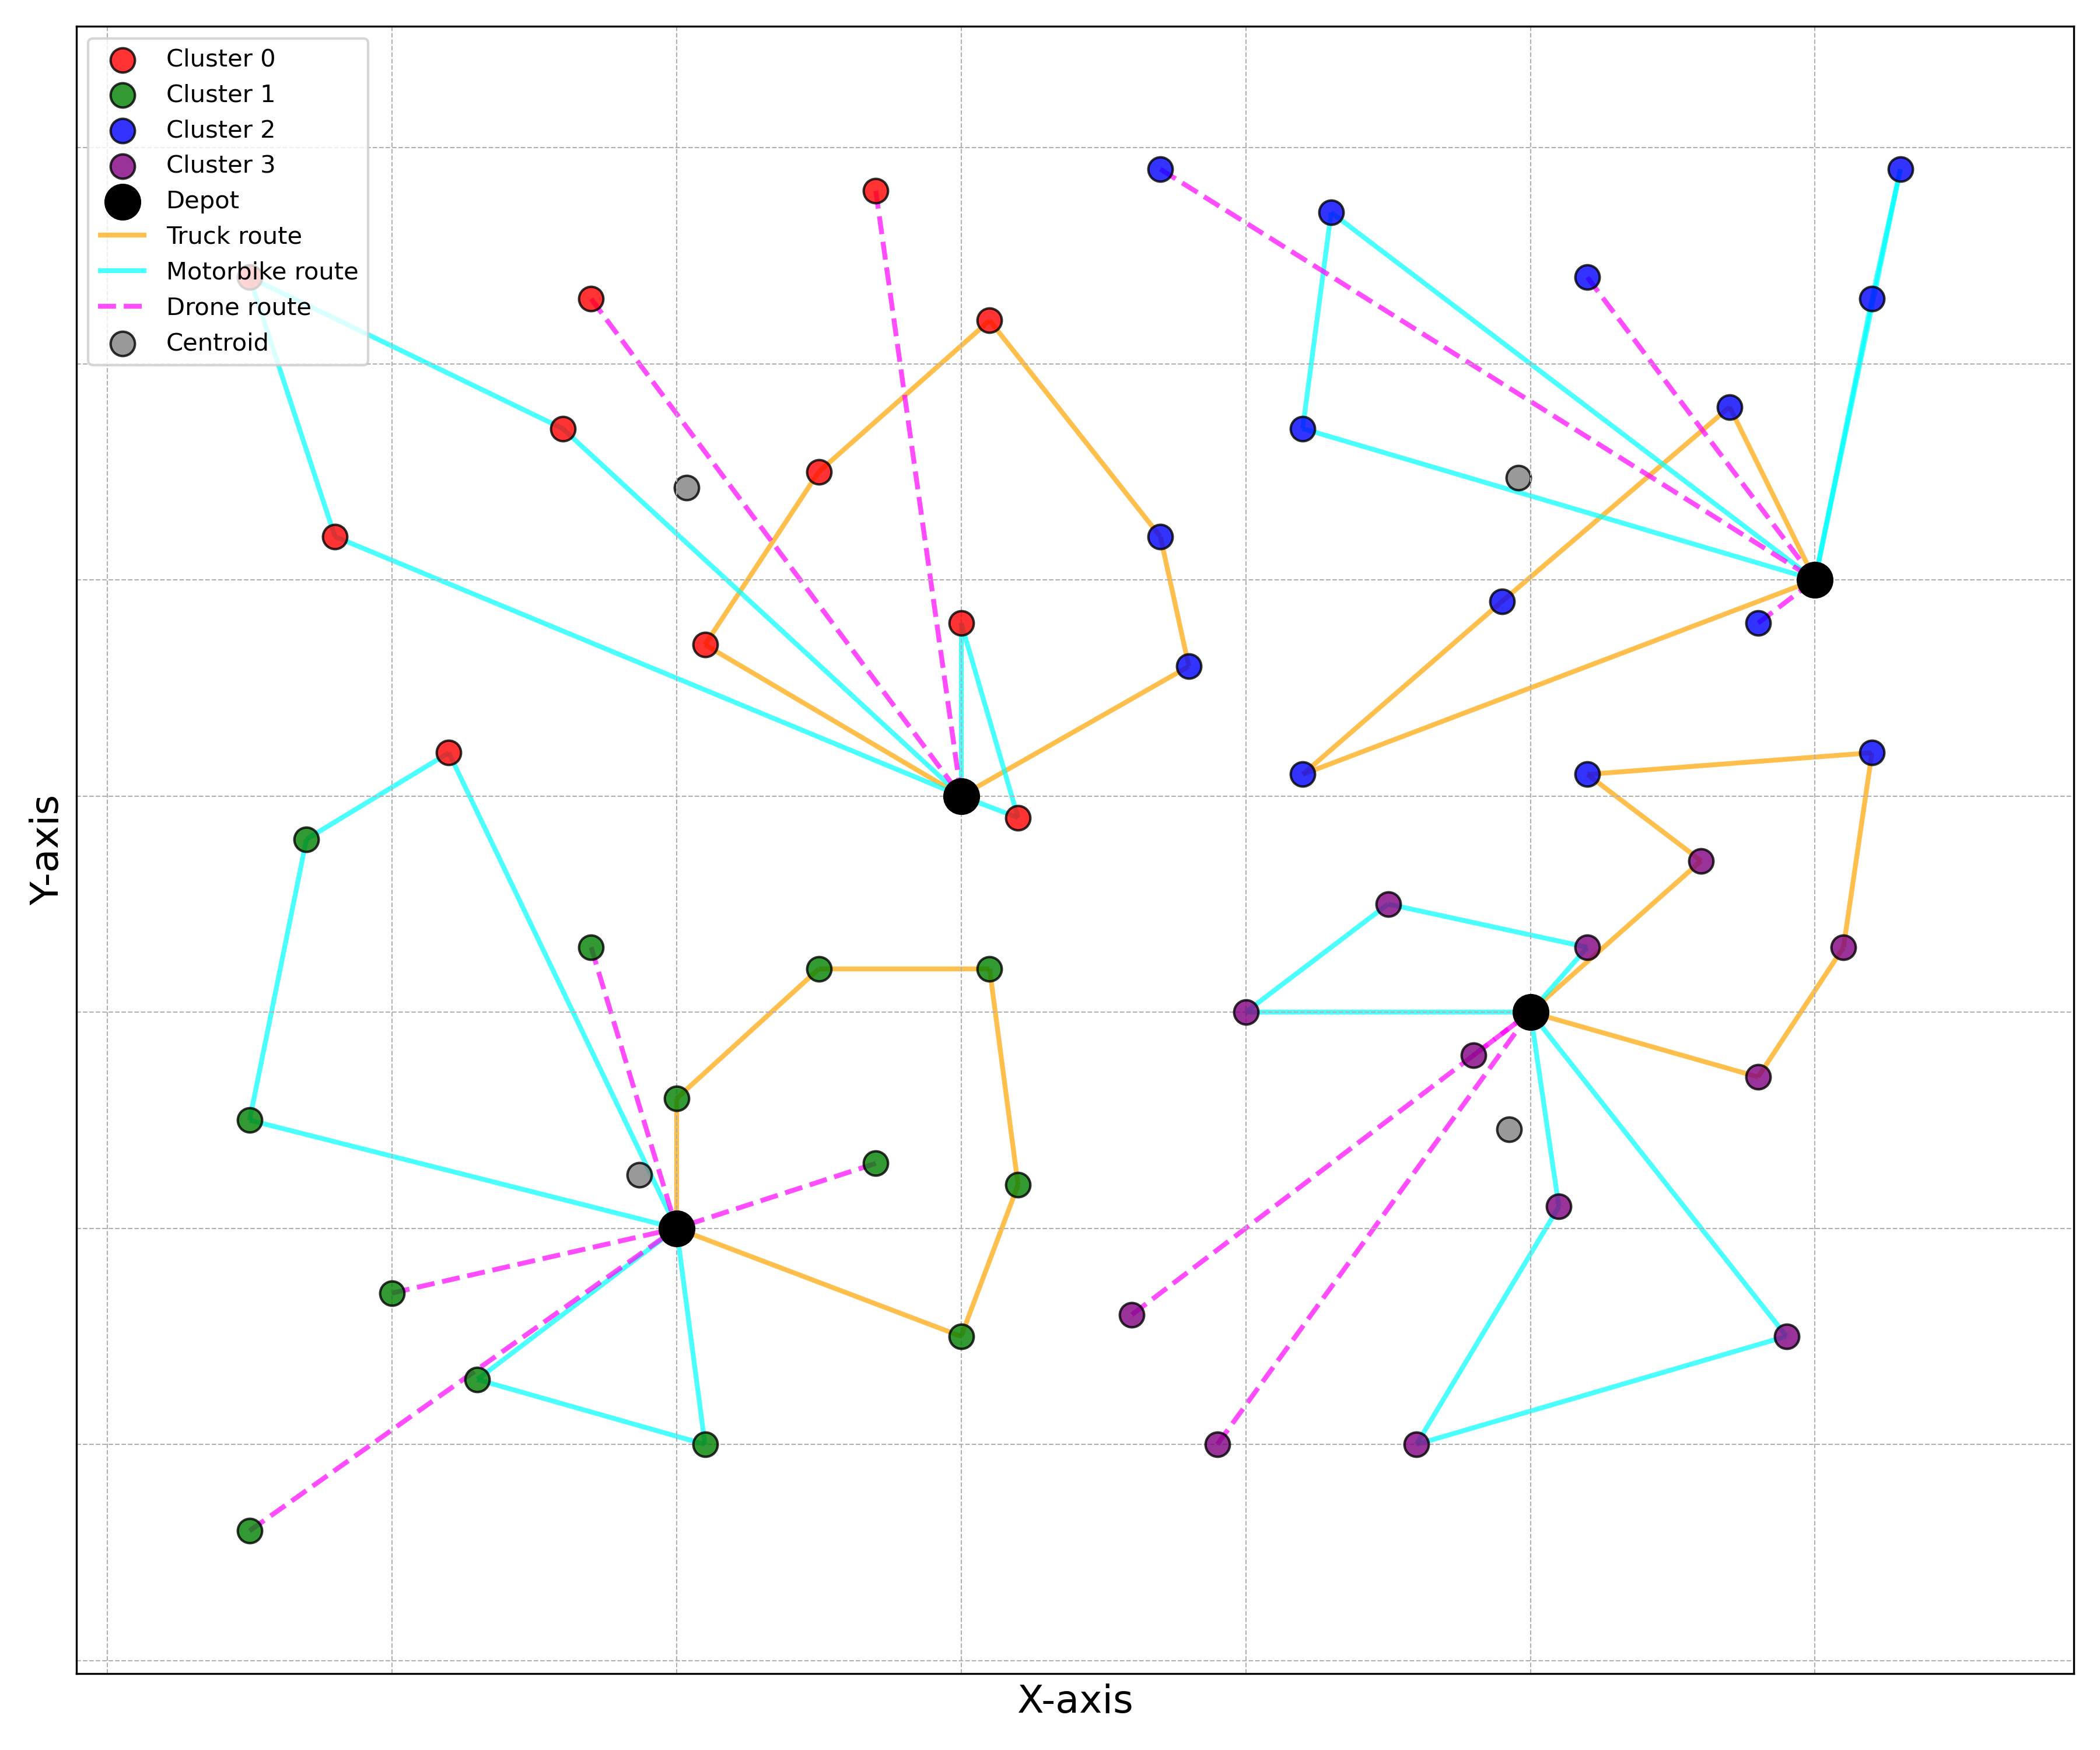
\includegraphics[width=\textwidth]{solution-p01}
		\centering
	\end{figure*}
	\clearpage
	\section{AACONC+}
	\begin{algorithm}
		\caption{AACONC+ Algorithm}
		\SetAlgoNlRelativeSize{-1}
		
		\SetKwProg{Fn}{Function}{}{}
		
		\Fn{AACONC+($V, n_{\text{ants}}, n_{\text{freq}}, n_{\text{size}}, n_{\text{sect}}, n_{\text{prim}}, T_{\text{update}}, \alpha, \beta, \rho_{\text{min}}, \rho_{\text{max}}, \delta$)}{
			$|R| = \infty$\;
			$iter = 0$\;
			Initialize pheromone matrices $\tau$\;
			
			\For{each $v_i \in V$}{
				$K(v_i)=$ CreateClusters($V, v_i, n_{\text{size}}, n_{\text{sect}}$)\;
			}
			
			\While{not terminated}{
				$|R_{\text{best}}| = \infty$\;
				$iter = iter + 1$\;
				
				\For{$a = 1$ to $n_{\text{ants}}$}{
					$R_a =$ AntSolution($V, K, \tau, \alpha, \beta$)\;
					
					\If{$|R_a| < |R_{\text{best}}|$}{
						$R_{\text{best}} = R_a$\;
					}
				}
				\If{$iter \mod n_{\text{freq}} = 0$}{
					$R_{\text{best}} =$ LocalOptimization($V, R_{\text{best}}$)\;
				}
				\If{$|R_{\text{best}}| < |R|$}{
					$R = R_{\text{best}}$\;
				}
				Update pheromone matrices $\tau$\;
				Calculate evaporation coefficient $\rho$\;
				Evaporate pheromone matrices $\tau$ using $\rho$\;
			}
			
			\textbf{return} $R$\;
		}
\end{algorithm}
\;
	
\begin{algorithm}
	\caption{createClusters}
	\SetKwProg{Fn}{Function}{}{}
	\Fn{createClusters($V^{(t_i)}, v_i, n_{size}, n_{sect}, n_{prim}$)}{
		
		$id = 1$\\
		$K_{id}^{(v_i)} = \emptyset$\\
		$V_{free} = V^{(t_i)}  - v_i$\\
		
		\For{j = 1 to $n_{sect}$}{
			Find closest vertex $v\in V_{free}$ to $v_i$ in sector $j$\\
			$K_{id}^{(v_i)} = K_{id}^{(v_i)} + \{v\}$\\
			$V_{free} = V_{free} - \{v\}$\\
		}
		\While{$V_{free} \neq \emptyset$}{
			\If{$|K_{id}^{(v_i)}| \geq n_{size}$}{
				$id = id + 1$\\
				$K_{id}^{(v_i)} = \emptyset$
			}
			Find closest vertex $v\in V_{free}$ to $v_i$\\
			$K_{id}^{(v_i)} = K_{id}^{(v_i)} + {v}$\\
			$V_{free} = V_{free} - {v}$\\
		}
		\textbf{return} $K^{(v_i)}$\;
	}
\end{algorithm}

\;
		
	\begin{algorithm}
		\caption{antSolution}
		
		\SetKwProg{Fn}{Function}{}{}
		
		\Fn{antSolution($V = \{D,C\}, K, \tau, \alpha, \beta$)}{
			$V_{free}$ = $C$\;
			
			\While{$V_{\text{free}} \neq \emptyset$}{
				$vt = $ selectVehicleType($V_{free}, K, \tau$)\\
				$d = $ selectDepot($vt, V_{free}, K^{(vt)}, \tau$)\\
				$v = $ selectVehicle($vt, d, V_{free}, K^{(vt)}, \tau$)\\
				
				$pos \leftarrow$ \text{vehicle's position}\
				
				$k = $ selectCluster($vt, d, v, V_{free}, K^{(pos)(vt)}, \tau, \alpha, \beta$)\
				
				$V_{candidates} = V_{\text{free}} \cap K_k^{(pos)(vt)}$\
				
				
				$c = $ selectCustomer($vt, d, pos, V_{candidates}, \tau, \alpha, \beta$)\\
				\uIf(//Drone serves customer and immediately returns to depot){vt = Drone}{
					$R_d^{vt} = R_d^{vt} + \{c\}$\\
					$R_d^{(vt)} = R_d^{(vt)} + \{d\}$\\
				}
				\Else{	
					\If{$v_{load} < c^{(demand)}$}{
						$R_d^{(vt)} = R_d^{(vt)} + \{d\}$\\
						$v_{load} = vt_{capacity}$\\
					}
					$R_d^{vt} = R_d^{vt} + \{c\}$\\
					$v_{pos} = \{c\}$\\
					$v_{load} = v_{load} - {c^{(demand)}}$\\
				}
				$V_{\text{free}} = V_{\text{free}} - \{c\}$\\
			}
			\ForEach(//Vehicles return to their depots){$d \in D \text{ and } vt\in VT$}{$R_d^{vt} = R_d^{vt} + \{d\}$}\
			\textbf{return} $R = \{R_1^1, R_2^1, ..., R_2^3, R_3^3, ...,R_D^{VT}\}$\
		}
		\end{algorithm}
\;
	
	
	\begin{algorithm}
		\caption{selectVehicle}
		\SetKwProg{Fn}{Function}{}{}
		
		\Fn{selectVehicle($vt, d, V_{free}, K^{(vt)}, \tau$)}{
				\For{each $v_i\in Vh^{(vt)(d)}$}{
					$V_{\text{cand}} = \emptyset$\\
					$pos \leftarrow$\text{vehicle's current location}\
					
					\For{\text{k = 1 to} $n_{prim}$}{
						$V_{cand} = V_{cand} + V_{free} \cap K_k^{(vt)(pos)}$\
					}
					
					$p(v_i) = \sum_{v_j \in V_{cand}} \tau_{v_{pos} v_j}^{(vt)(d)}$\
				}
			$p_{sum} = \sum_{v_i \in V^{(vt)(d)}} p(v_i)$\\
			$p(v_i) = p(v_i)\div p_{sum}$\\
			Select $v_i\in Vh^{(vt)(d)}$ based on probabilities $p(v_i)$ using roulette wheel\\
			\textbf{return} $v_i$\;
		}
		
	\end{algorithm}

\;
	\clearpage
	\onecolumn
	\section{Instances}
	% Please add the following required packages to your document preamble:
% \usepackage{booktabs}
% \usepackage{graphicx}
\begin{table}[h]
	\centering
	\begin{minipage}{0.7\columnwidth}
	\centering
	\caption{MD-mfcmTSP Instances}
	\resizebox{\columnwidth}{!}{%
		\begin{tabular}{@{}ccccccc@{}}
			\toprule
			\textbf{Instance} & \textbf{Customers} & \textbf{Depots} & \textbf{Dimensions} & \textbf{$C^{Truck}$} & \textbf{$C^{UAV}$} \\
			\midrule
			1 & 50 & 4 & 3150m x 3450m & 46 & 42 \\
			\midrule
			2 & 50 & 4 & 3150m x 3450m & 46 & 40 \\
			\midrule
			3 & 75 & 5 & 3500m x 3800m & 64 & 62\\
			\midrule
			4 & 100 & 2 & 3350m x 3850m & 88 & 87 \\
			\midrule
			5 & 100 & 2 & 3350m x 3850m & 91 & 82 \\
			\midrule
			6 & 100 & 3 & 3350m x 3850m & 91 & 85 \\
			\midrule
			7 & 100 & 4 & 3350m x 3850m & 97 & 83 \\
			\midrule
			8 & 249 & 2 & 9900m x 9800m & 219 & 215 \\
			\midrule
			9 & 249 & 3 & 9900m x 9800m & 224 & 212 \\
			\midrule
			10 & 249 & 4 & 9900m x 9800m & 223 & 221 \\
			\midrule
			11 & 249 & 5 & 10500m x 5000m & 222 & 208 \\
			\midrule
			12 & 500 & 4 & 7500m x 7500m & 461 & 425 \\
			\midrule
			13 & 500 & 4 & 7500m x 7500m & 448 & 436 \\
			\midrule
			14 & 500 & 5 & 7500m x 7500m & 458 & 413 \\
			\midrule
			15 & 1000 & 4 & 10000m x 10000m & 903 & 855 \\
			\midrule
			16 & 1000 & 6 & 10000m x 10000m & 887 & 842 \\
			\bottomrule
		\end{tabular}%
	}
	\label{tab:instances_table}
\end{minipage}
\end{table}\;
	\clearpage
	\begin{figure}[h!]
		\centering
		\caption{Regular Layout Instance}
		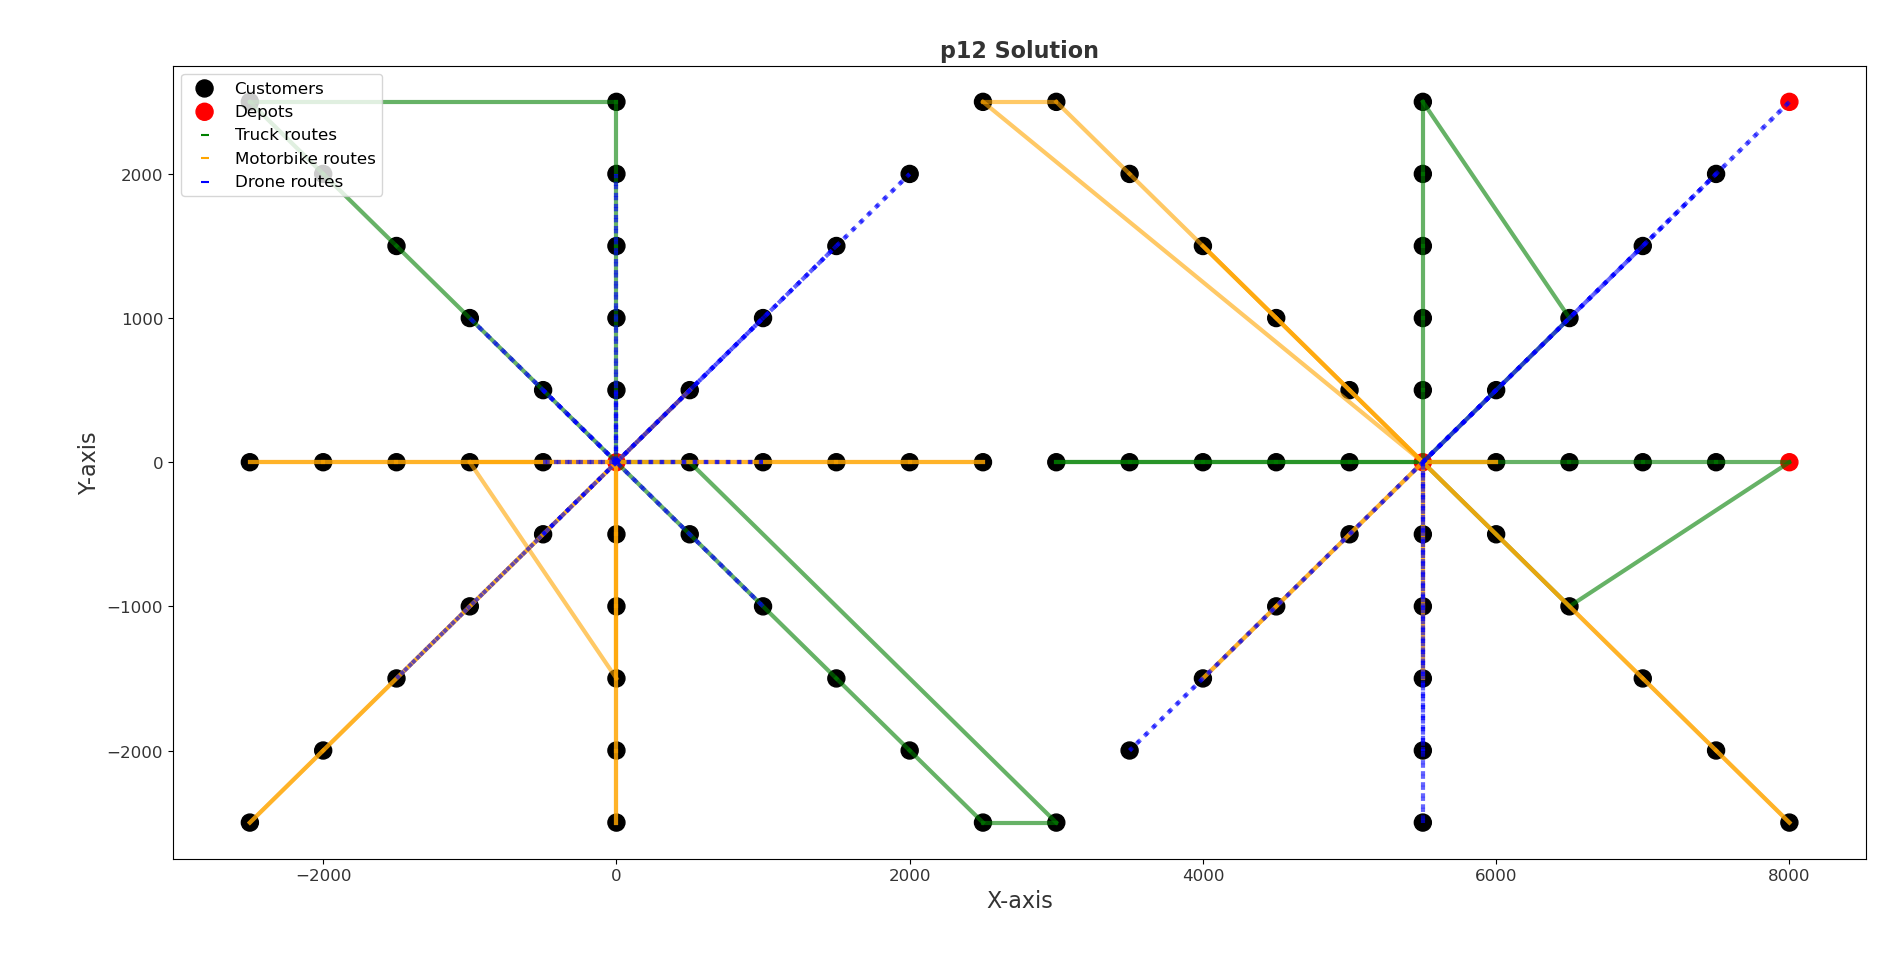
\includegraphics[width=\columnwidth]{p12_aco-1}
	\end{figure}

	\onecolumn
	\section{Results}
	\subsection{New heuristic vs old heuristic}
	\textbf{mfcmTSP heuristic (original) : } Finds and swaps the minimum cost route in each iteration \\ \;
	\\
	\par
	\textbf{MD-mfcmTSP heuristic (v1) : } Finds and swaps the route which minimizes the depot's makespan in each iteration \\ \;
	\begin{figure*}[hb!]
		\centering
		\caption{Comparison between new and original heuristic}
		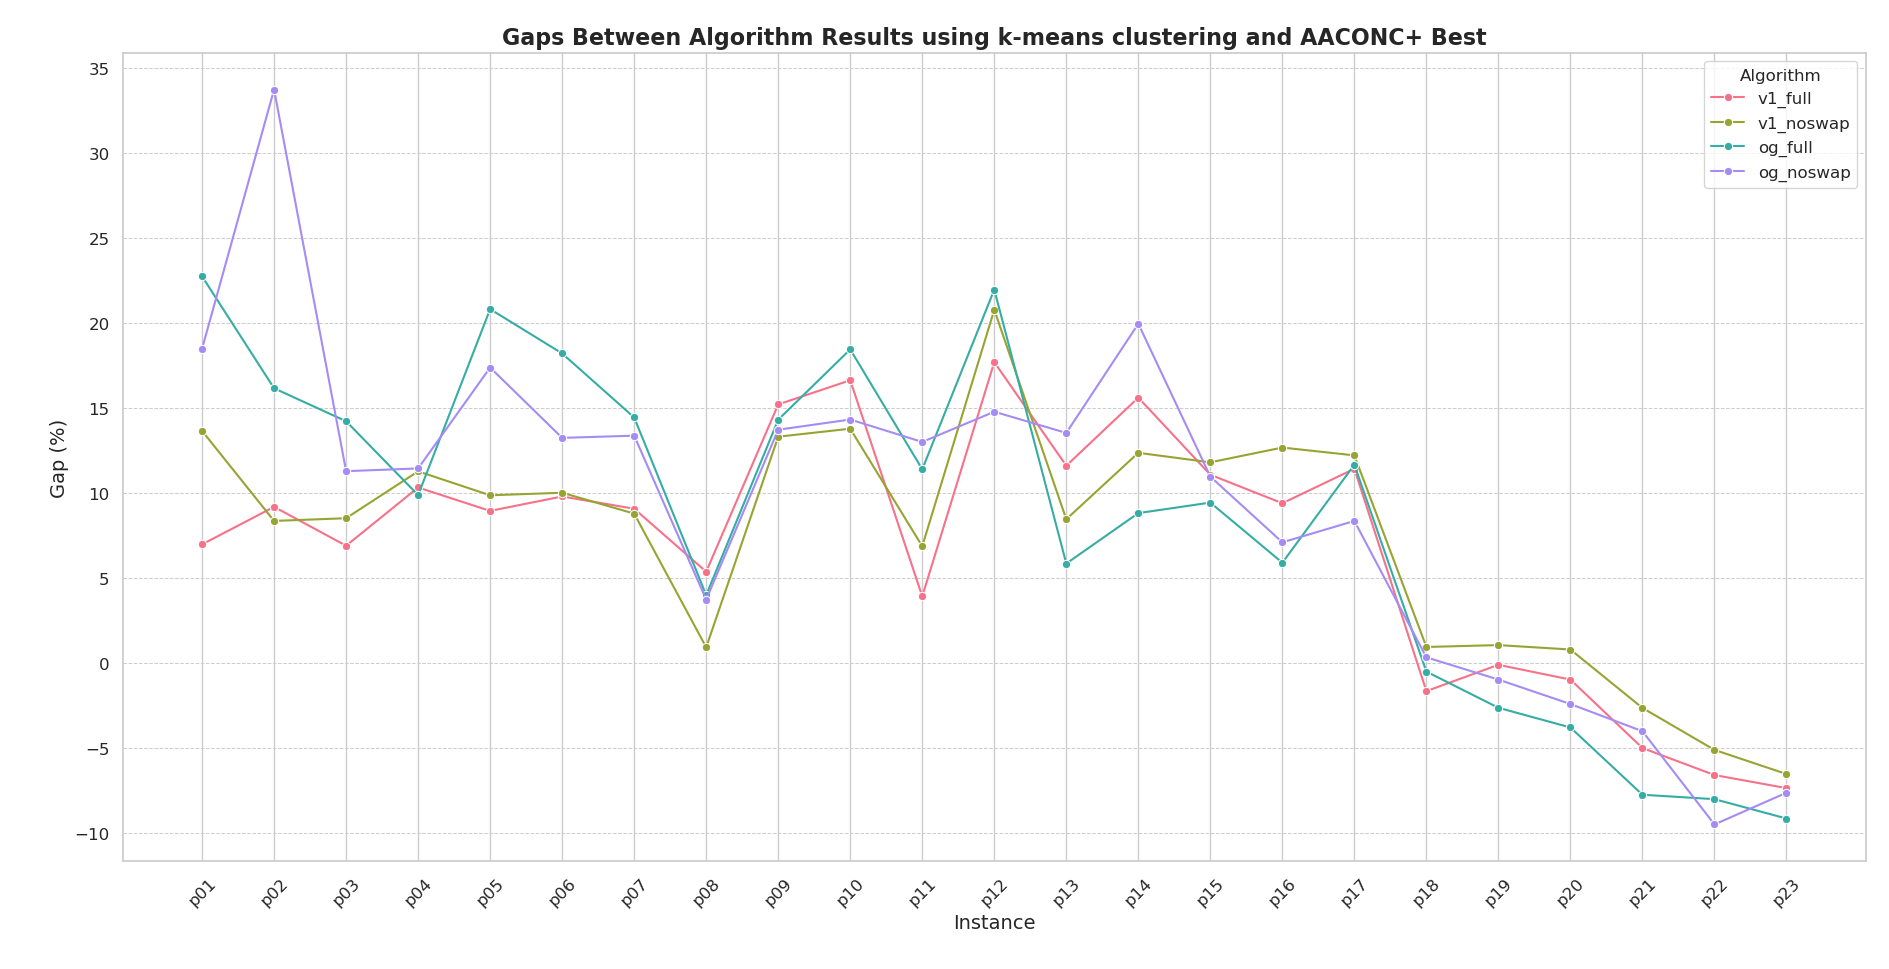
\includegraphics[width=\textwidth]{heuristics_comp_gaps_lineGraph_kmeans}
	\end{figure*}
	\begin{figure*}[hb!]
		\centering
		\caption{Comparison between new and original heuristic}
		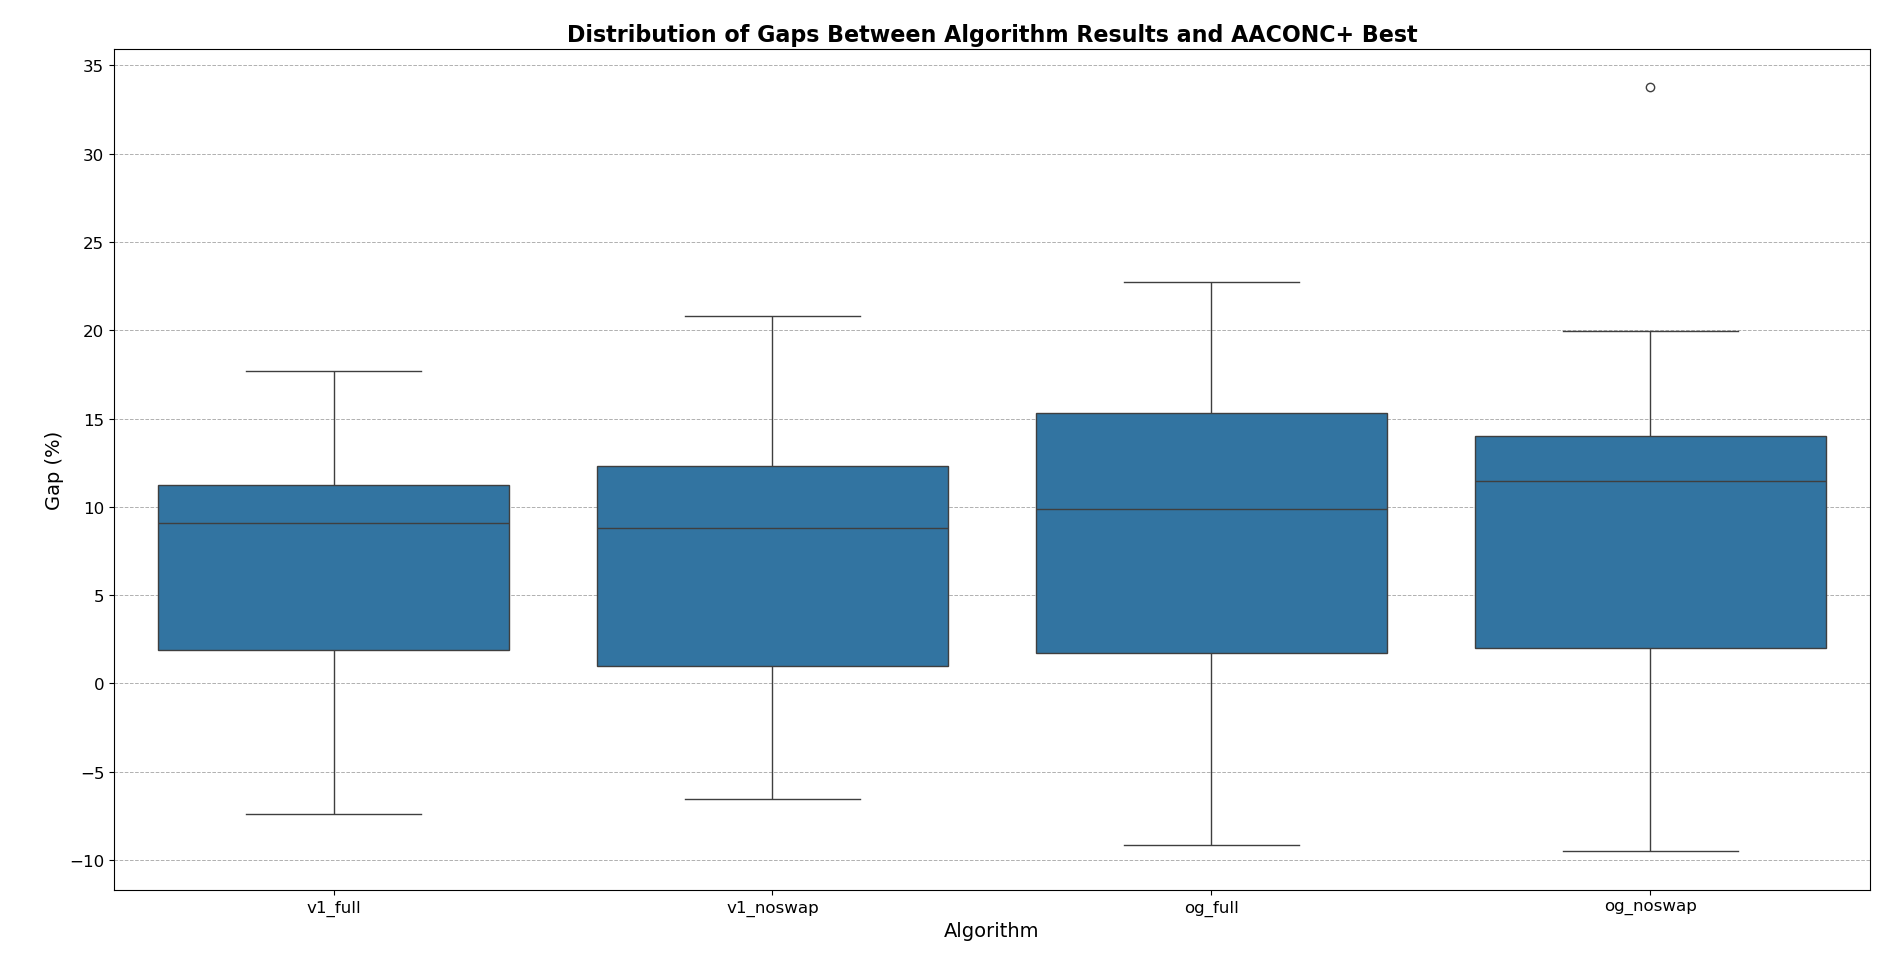
\includegraphics[width=\textwidth]{heuristics_comp_gaps_boxGraph_kmeans}
	\end{figure*}
	\begin{figure*}[hb!]
		\centering
		\caption{Comparison between new and original heuristic}
		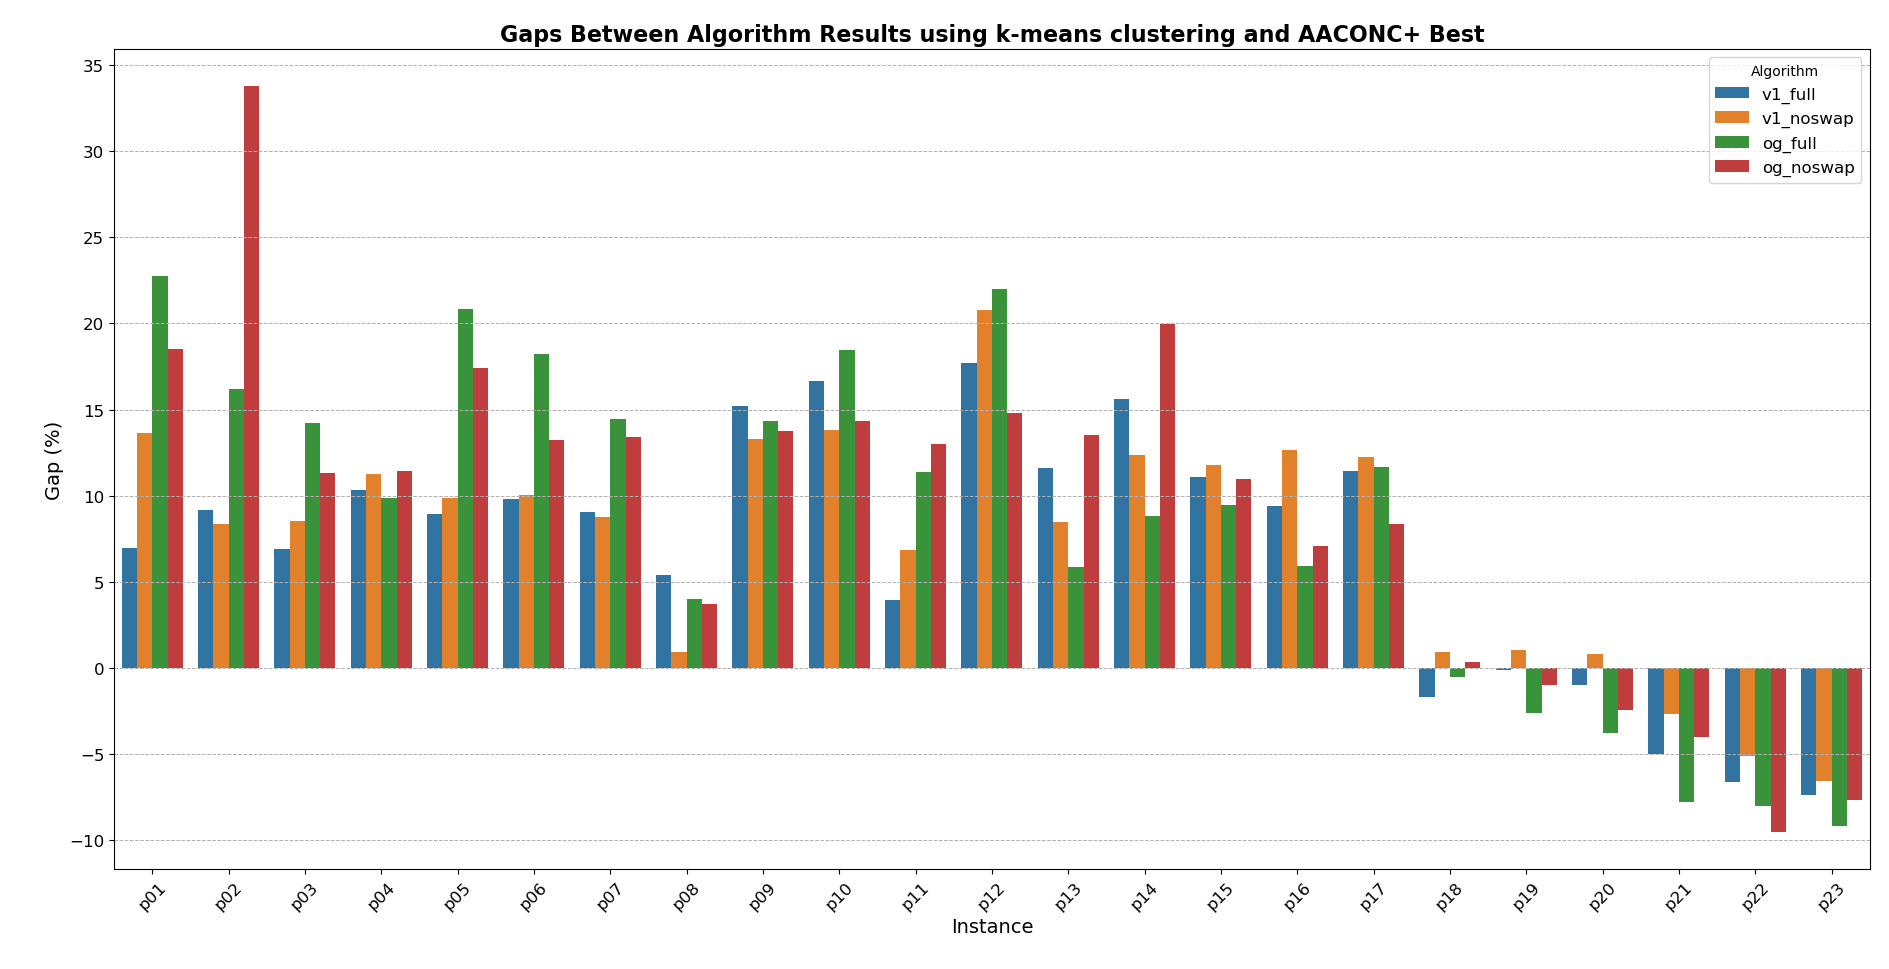
\includegraphics[width=\textwidth]{heuristics_comp_gaps_barGraph_kmeans}
	\end{figure*}
	
	
	
	\clearpage
	\section{MD-mfcmTSP Results Analysis}
	\subsection{Local optimization impact on the heuristic}
	\subsubsection{Proximity clustering}
	% Please add the following required packages to your document preamble:
% \usepackage{booktabs}
% \usepackage{graphicx}
\begin{table*}[!ht]
	\centering
	\caption{Local optimization impact on heuristic using proximity clustering}
	\resizebox{\textwidth}{!}{%
		\begin{tabular}{@{}cccccccccc@{}}
			\toprule
			\textbf{Instance} & \textbf{Best} & \textbf{Full Local Opt} & \textbf{gap(\%)} & \textbf{No Local Opt} & \textbf{gap(\%)} & \textbf{Final Only} & \textbf{gap(\%)} & \textbf{Swap Only} & \textbf{gap(\%)} \\ 
			\midrule
			p01-C & 215.15 & 217.42 & 1.06 & 334.04 & 55.26 & \textbf{215.15} & 0.00 & 173.96 & 27.33 \\ \midrule
			p02-C & 218.4 & 219.20 & 0.37 & 308.83 & 41.41 & \textbf{218.40} & 0.00 & 289.58 & 32.59 \\ \midrule
			p03-C & 202.43 & 214.84 & 6.13 & 253.18 & 25.07 & \textbf{202.43} & 0.00 & 255.52 & 26.23 \\ \midrule
			p04-C & 668.81 & \textbf{668.81} & 0.00 & 779.34 & 16.53 & 711.80 & 6.43 & 691.62 & 3.41 \\ \midrule
			p05-C & 630.78 & \textbf{630.78} & 0.00 & 726.62 & 15.19 & 655.4 & 3.90 & 697.86 & 10.63 \\ \midrule
			p06-C & 431.32 & 435.42 & 0.95 & 650.32 & 50.77 & \textbf{431.32} & 0.00 & 564.79 & 30.94 \\ \midrule
			p07-C & 309.48 & \textbf{309.48} & 0.00 & 350.77 & 13.34 & 349.19 & 12.83 & 366.51 & 18.43 \\ \midrule
			p08-C & 3079.58 & 3333.93 & 8.26 & 3321.63 & 7.86 & \textbf{3079.58} & 0.00 & 3428.15 & 11.32 \\ \midrule
			p09-C & 1917.82 & \textbf{1917.82} & 0.00 & 2429.24 & 26.67 & 2102.98 & 9.65 & 2303.70 & 20.12 \\ \midrule
			p10-C & 1493.13 & \textbf{1493.13} & 0.00 & 1864.23 & 24.85 & 1525.37 & 2.16 & 1706.14 & 14.27 \\ \midrule
			p11-C & 1101.33 & 1145.75 & 4.03 & 1239.36 & 12.53 & \textbf{1101.33} & 0.00 & 1276.59 & 15.91 \\ \midrule
			p12-C & 1273.77 & \textbf{1273.77} & 0.00 & 1356.09 & 6.46 & 1307.11 & 2.62 & \textbf{1273.77} & 0.00 \\ \midrule
			p13-C & 1191.96 & 1226.63 & 2.91 & 1455.87 & 22.14 & \textbf{1191.96} & 0.00 & 1259.97 & 5.71 \\ \midrule
			p14-C & 1248.53 & 1284.73 & 2.90 & 1413.87 & 13.24 & \textbf{1248.53} & 0.00 & 1302.34 & 4.31 \\ \midrule
			p15-C & 1347.67 & \textbf{1347.67} & 0.00 & 1508.50 & 11.93 & 1355.08 & 0.55 & 1375.95 & 2.10 \\ \midrule
			p16-C & 1289.29 & \textbf{1289.29} & 0.00 & 1448.53 & 12.35 & 1328.00 & 3.00 & \textbf{1289.29} & 0.00 \\ \midrule
			p17-C & 1282.38 & 1320.91 & 3.00 & 1375.55 & 7.27 & \textbf{1282.38} & 0.00 & 1320.91 & 3.00 \\ \midrule
			p18-C & 1260.24 & \textbf{1260.24} & 0.00 & 1446.92 & 14.81 & 1317.54 & 4.55 & 1339.83 & 6.32 \\ \midrule
			p19-C & 1266.92 & \textbf{1266.92} & 0.00 & 1406.13 & 10.99 & 1289.95 & 1.82 & 1301.62 & 2.74 \\ \midrule
			p20-C & 1323.1 & \textbf{1323.10} & 0.00 & 1429.00 & 8.00 & 1338.42 & 1.16 & 1351.39 & 2.14 \\ \midrule
			p21-C & 1309.14 & 1363.18 & 4.13 & 1470.03 & 12.29 & \textbf{1309.14} & 0.00 & 1363.18 & 4.13 \\ \midrule
			p22-C & 1295.67 & \textbf{1295.67} & 0.00 & 1465.74 & 13.13 & 1351.96 & 4.34 & 1306.6 & 0.84 \\ \midrule
			p23-C & 1252.36 & \textbf{1252.36} & 0.00 & 1396.11 & 11.48 & 1262.65 & 0.82 & 1254.42 & 0.16 \\ \midrule
			\textbf{AVG} & 1113.44 & \textbf{1134.39} & \textbf{1.46} & 1279.56 & 18.85 & 1138.07 & 2.34 & 1199.72 & 10.54 \\ \bottomrule
		\end{tabular}%
	}
\end{table*}\;
	\begin{figure*}[hb!]
		\centering
		\caption{Gaps to full local optimization (proximity clustering)}
		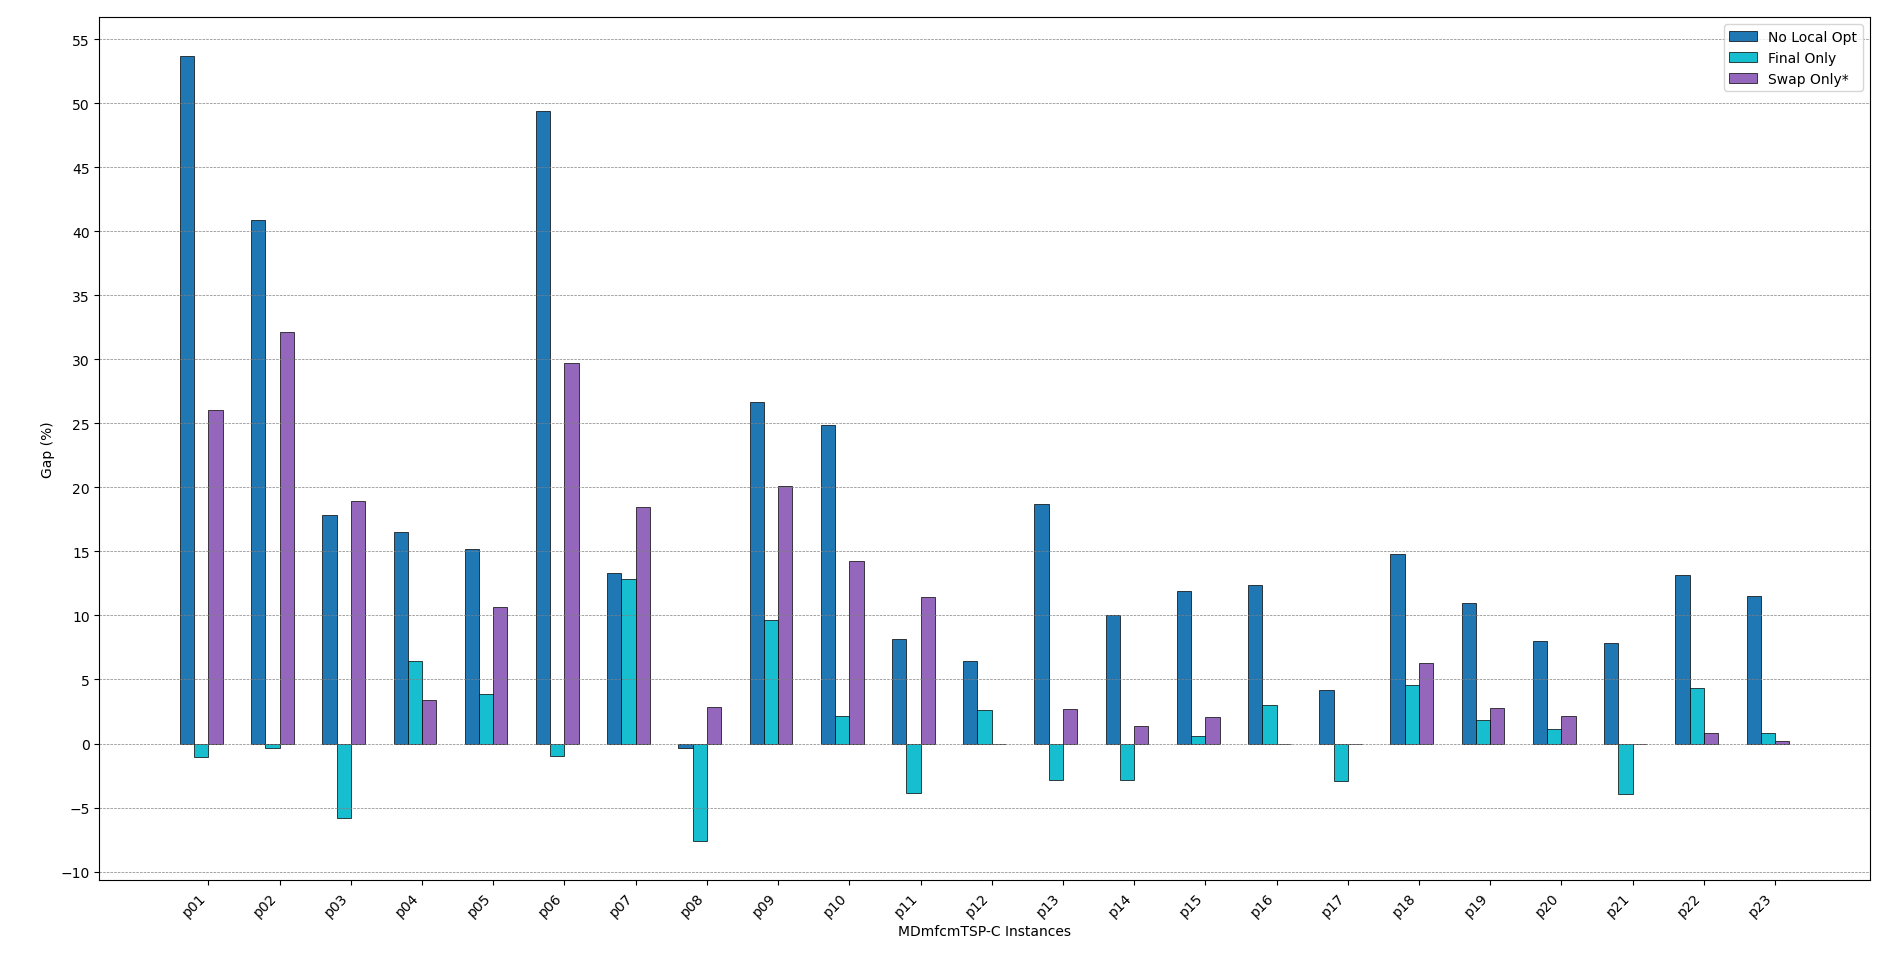
\includegraphics[width=\textwidth]{local_opt_comp_to_full_proximity}
	\end{figure*}
	\begin{figure*}[hb!]
		\centering
		\caption{Results using proximity clustering}
		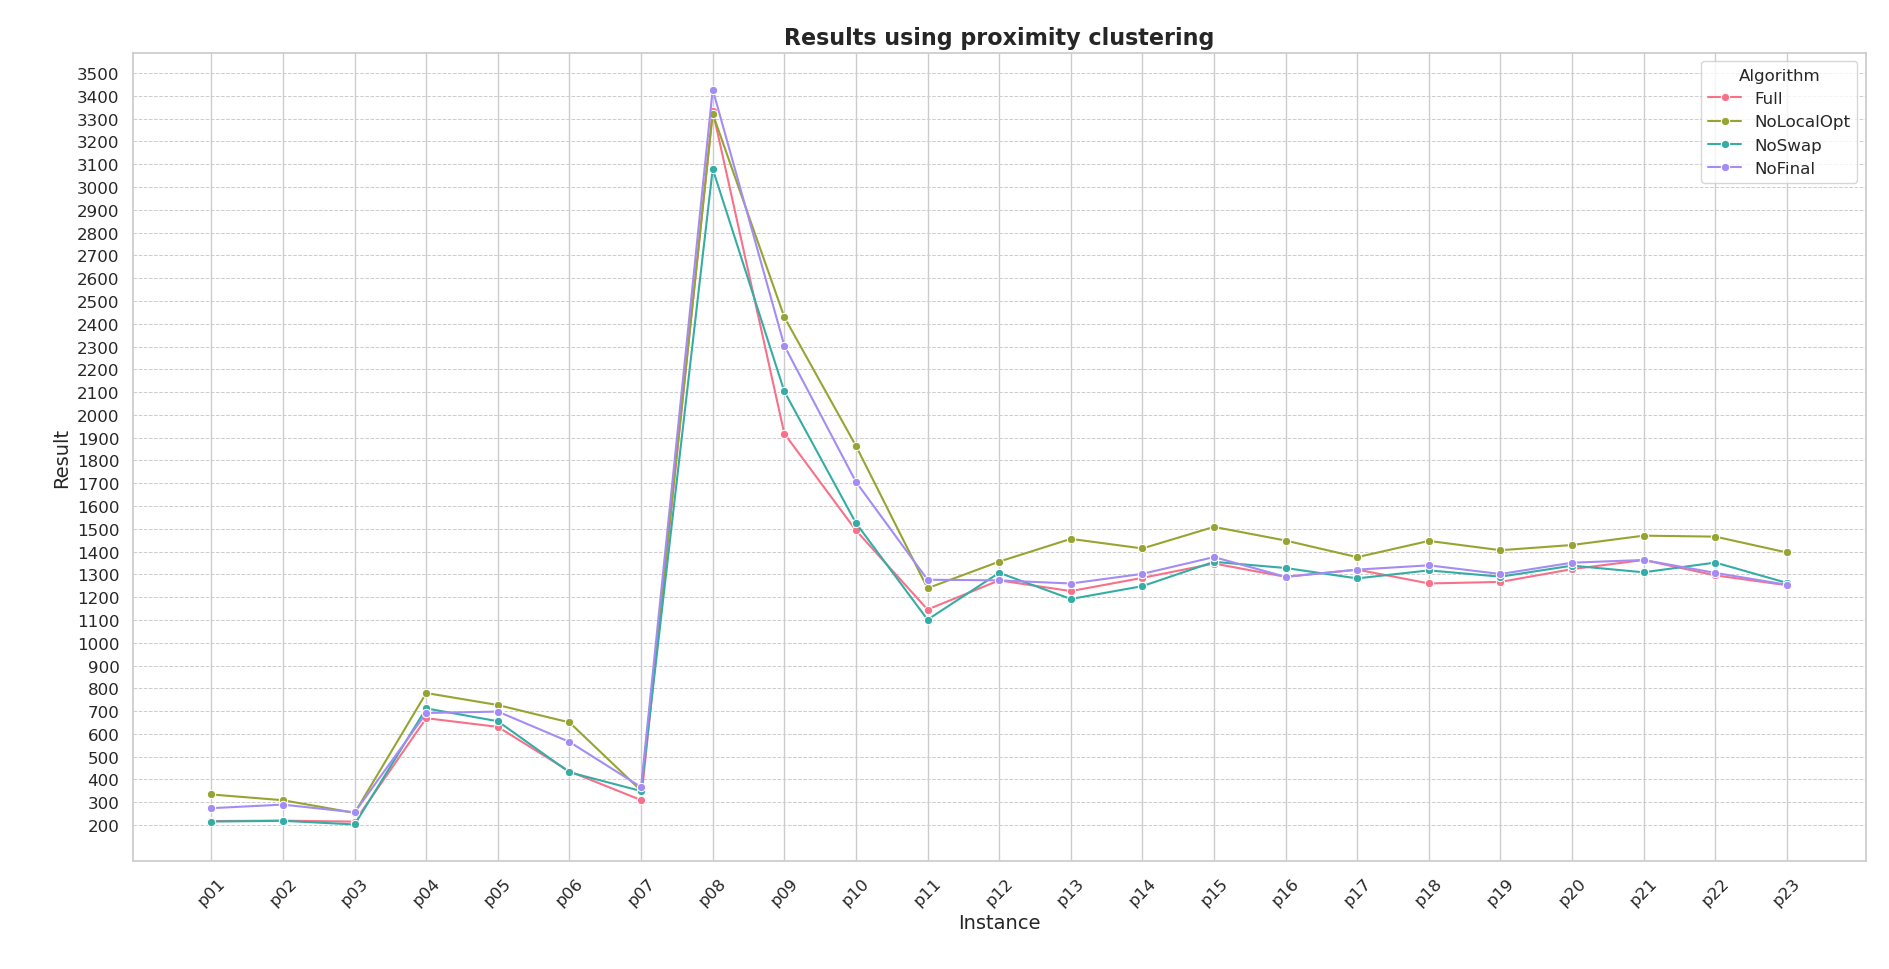
\includegraphics[width=\textwidth]{Results_proximity}
	\end{figure*}

	\clearpage
	\subsubsection{k-means clustering}
	% Please add the following required packages to your document preamble:
% \usepackage{booktabs}
% \usepackage{graphicx}
\begin{table*}[!ht]
		\centering
	\caption{Local optimization impact on heuristic using k-means clustering}
	\resizebox{\textwidth}{!}{%
		\begin{tabular}{@{}cccccccccc@{}}
			\toprule
			\textbf{Instance} & \textbf{Best} & \textbf{Full Local Opt} & \textbf{gap(\%)} & \textbf{No Local Opt} & \textbf{gap(\%)} & \textbf{Final Only} & \textbf{gap(\%)} & \textbf{Swap Only} & \textbf{gap(\%)} \\ \midrule
			p01 & \textbf{191.03} & \textbf{191.03} & 0.00 & 225.72 & 18.16 & 202.96 & 6.25 & 201.60 & 5.53 \\
			\midrule
			p02 & \textbf{187.17} & 188.60 & 0.76 & 209.39 & 11.87 & \textbf{187.17} & 0.00 & 198.02 & 5.80 \\
			\midrule
			p03 & \textbf{185.82} & \textbf{185.82} & 0.00 & 200.64 & 7.98 & 188.63 & 1.51 & 198.01 & 6.56 \\
			\midrule
			p04 & \textbf{694.96} & \textbf{694.96} & 0.00 & 807.71 & 16.22 & 700.95 & 0.86 & \textbf{694.96} & 0.00 \\
			\midrule
			p05 & \textbf{624.33} & \textbf{624.33} & 0.00 & 695.79 & 11.45 & 629.61 & 0.85 & 642.77 & 2.95 \\
			\midrule
			p06 & \textbf{416.25} & \textbf{416.25} & 0.00 & 492.31 & 18.27 & 417.09 & 0.20 & 456.81 & 9.74 \\
			\midrule
			p07 & \textbf{313.57} & 314.41 & 0.27 & 359.30 & 14.58 & \textbf{313.57} & 0.00 & 339.09 & 8.14 \\
			\midrule
			p08 & \textbf{3051.63} & 3186.02 & 4.40 & 3288.45 & 7.76 & \textbf{3051.63} & 0.00 & 3256.46 & 6.71 \\
			\midrule
			p09 & \textbf{1932.21} & 1964.49 & 1.67 & 2099.99 & 8.68 & \textbf{1932.21} & 0.00 & 2031.19 & 5.12 \\
			\midrule
			p10 & \textbf{1463.63} & 1500.38 & 2.51 & 1636.23 & 11.79 & \textbf{1463.63} & 0.00 & 1658.74 & 13.33 \\
			\midrule
			p11 & \textbf{1031.09} & \textbf{1031.09} & 0.00 & 1209.73 & 17.33 & 1060.37 & 2.84 & 1080.39 & 4.78 \\
			\midrule
			p12 & \textbf{1273.77} & \textbf{1273.77} & 0.00 & 1356.09 & 6.46 & 1307.11 & 2.62 & \textbf{1273.77} & 0.00 \\
			\midrule
			p13 & \textbf{1191.96} & 1226.63 & 2.91 & 1455.87 & 22.14 & \textbf{1191.96} & 0.00 & 1259.97 & 5.71 \\
			\midrule
			p14 & \textbf{1248.53} & 1284.73 & 2.90 & 1413.87 & 13.24 & \textbf{1248.53} & 0.00 & 1302.34 & 4.31 \\
			\midrule
			p15 & \textbf{1295.23} & \textbf{1295.23} & 0.00 & 1434.72 & 10.77 & 1303.76 & 0.66 & \textbf{1295.23} & 0.00 \\
			\midrule
			p16 & \textbf{1289.29} & \textbf{1289.29} & 0.00 & 1436.36 & 11.41 & 1328.00 & 3.00 & \textbf{1289.29} & 0.00 \\
			\midrule
			p17 & \textbf{1273.39} & \textbf{1273.39} & 0.00 & 1375.55 & 8.02 & 1282.38 & 0.71 & 1283.38 & 0.78 \\
			\midrule
			p18 & \textbf{1211.56} & \textbf{1211.56} & 0.00 & 1369.81 & 13.06 & 1243.53 & 2.64 & 1280.85 & 5.72 \\
			\midrule
			p19 & \textbf{1248.93} & \textbf{1248.93} & 0.00 & 1384.13 & 10.83 & 1263.35 & 1.15 & 1281.68 & 2.62 \\
			\midrule
			p20 & \textbf{1234.12} & \textbf{1234.12} & 0.00 & 1389.60 & 12.60 & 1256.25 & 1.79 & 1267.53 & 2.71 \\
			\midrule
			p21 & \textbf{1231.23} & \textbf{1231.23} & 0.00 & 1354.91 & 10.05 & 1261.89 & 2.49 & 1278.10 & 3.81 \\
			\midrule
			p22 & \textbf{1230.99} & \textbf{1230.99} & 0.00 & 1379.49 & 12.06 & 1250.49 & 1.58 & 1265.17 & 2.78 \\
			\midrule
			p23 & \textbf{1222.63} & \textbf{1222.63} & 0.00 & 1363.52 & 11.52 & 1233.67 & 0.90 & 1250.29 & 2.26 \\
			\midrule
			Average & \textbf{1088.84} & 1100.86 & 0.67 & 1214.75 & 12.45 & 1100.81 & 1.31 & 1134.16 & 4.32 \\
			\bottomrule
		\end{tabular}%
	}

\end{table*}
\;
	\begin{figure*}[hb!]
		\caption{Comparison to full local optimization (k-means clustering)}
		\centering
		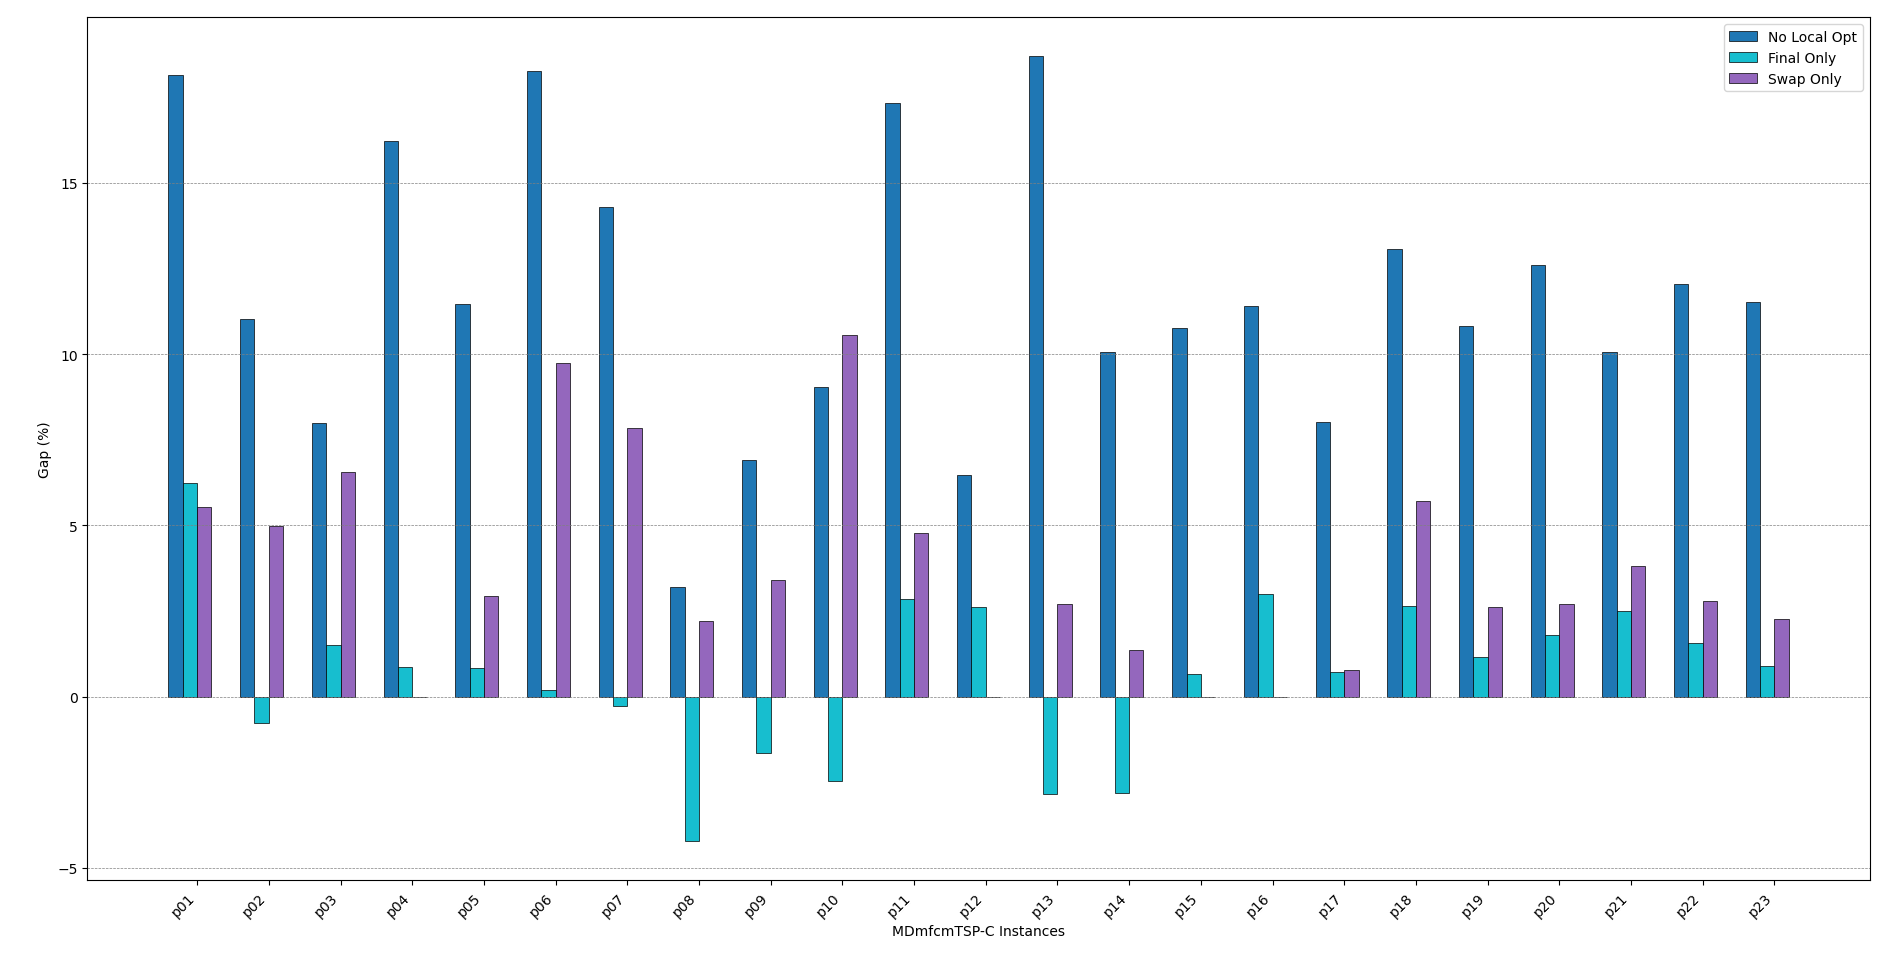
\includegraphics[width=\textwidth]{local_opt_comp_to_full_kmeans}
	\end{figure*}
	\begin{figure*}[hb!]
		\caption{Results using k-means clustering}
		\centering
		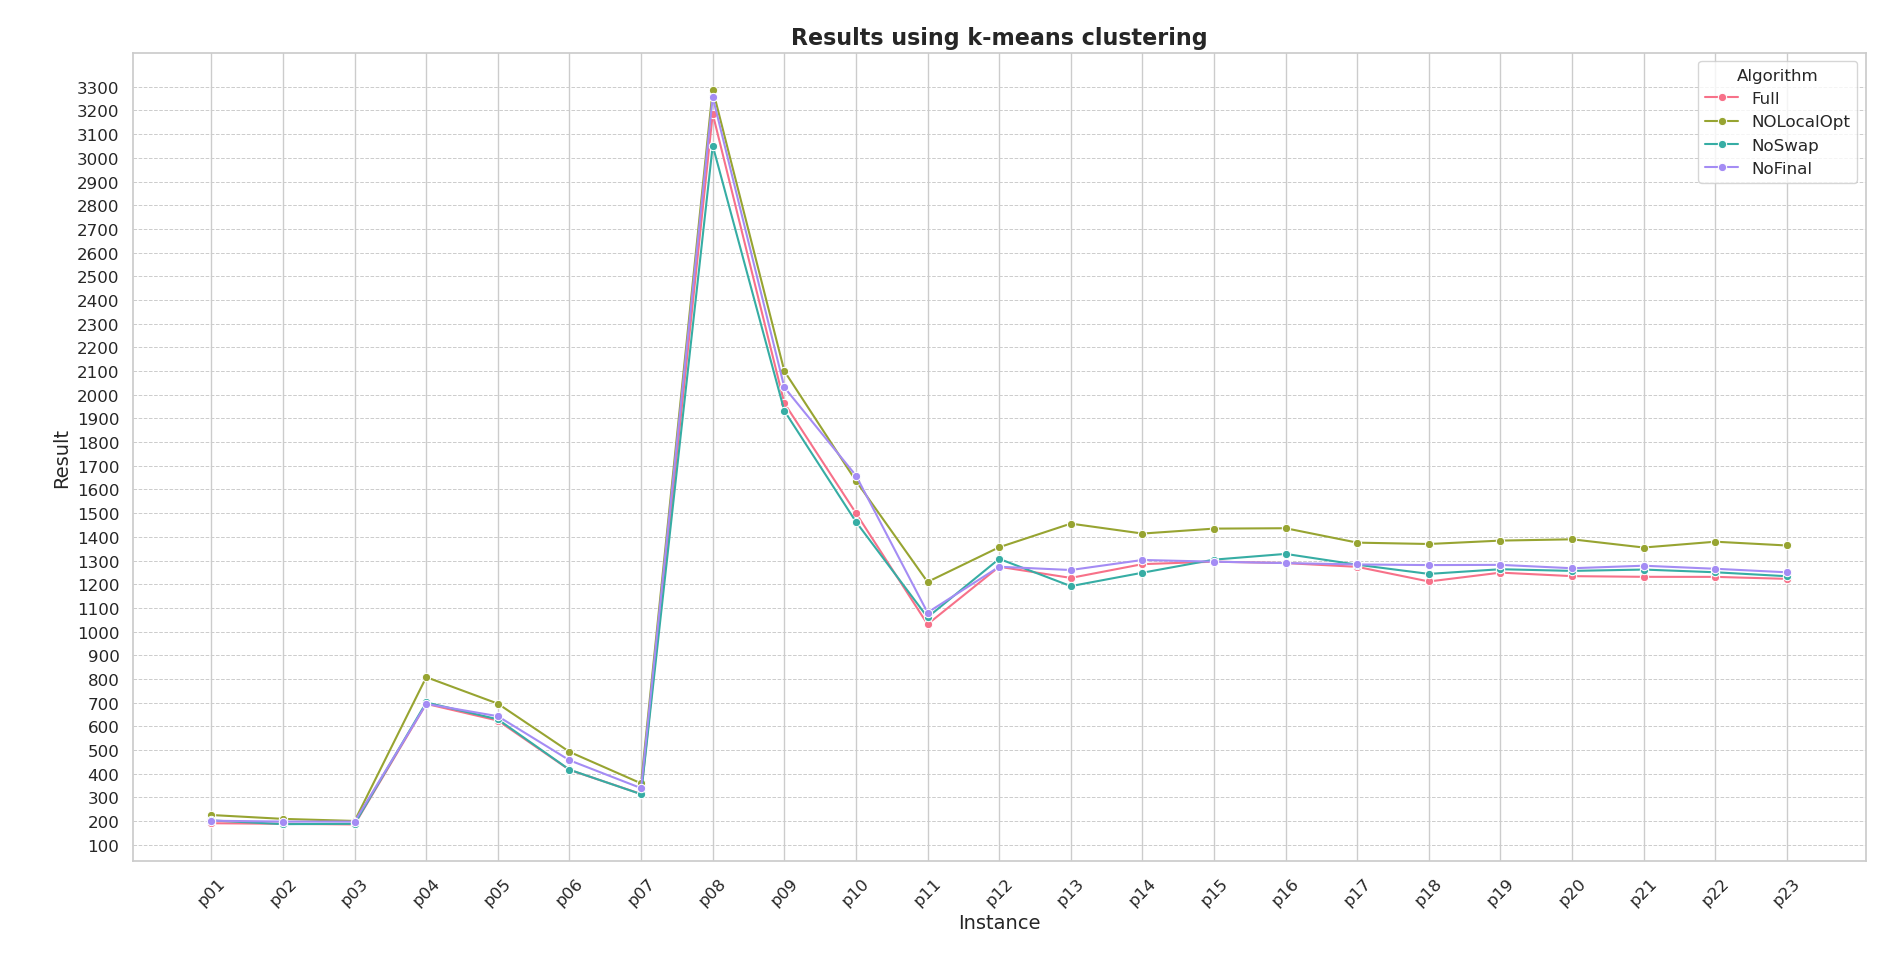
\includegraphics[width=\textwidth]{Results_kmeans}
	\end{figure*}
	\begin{figure*}[hb!]
		\caption{Local optimization impact on computational time (k-means)}
		\centering
		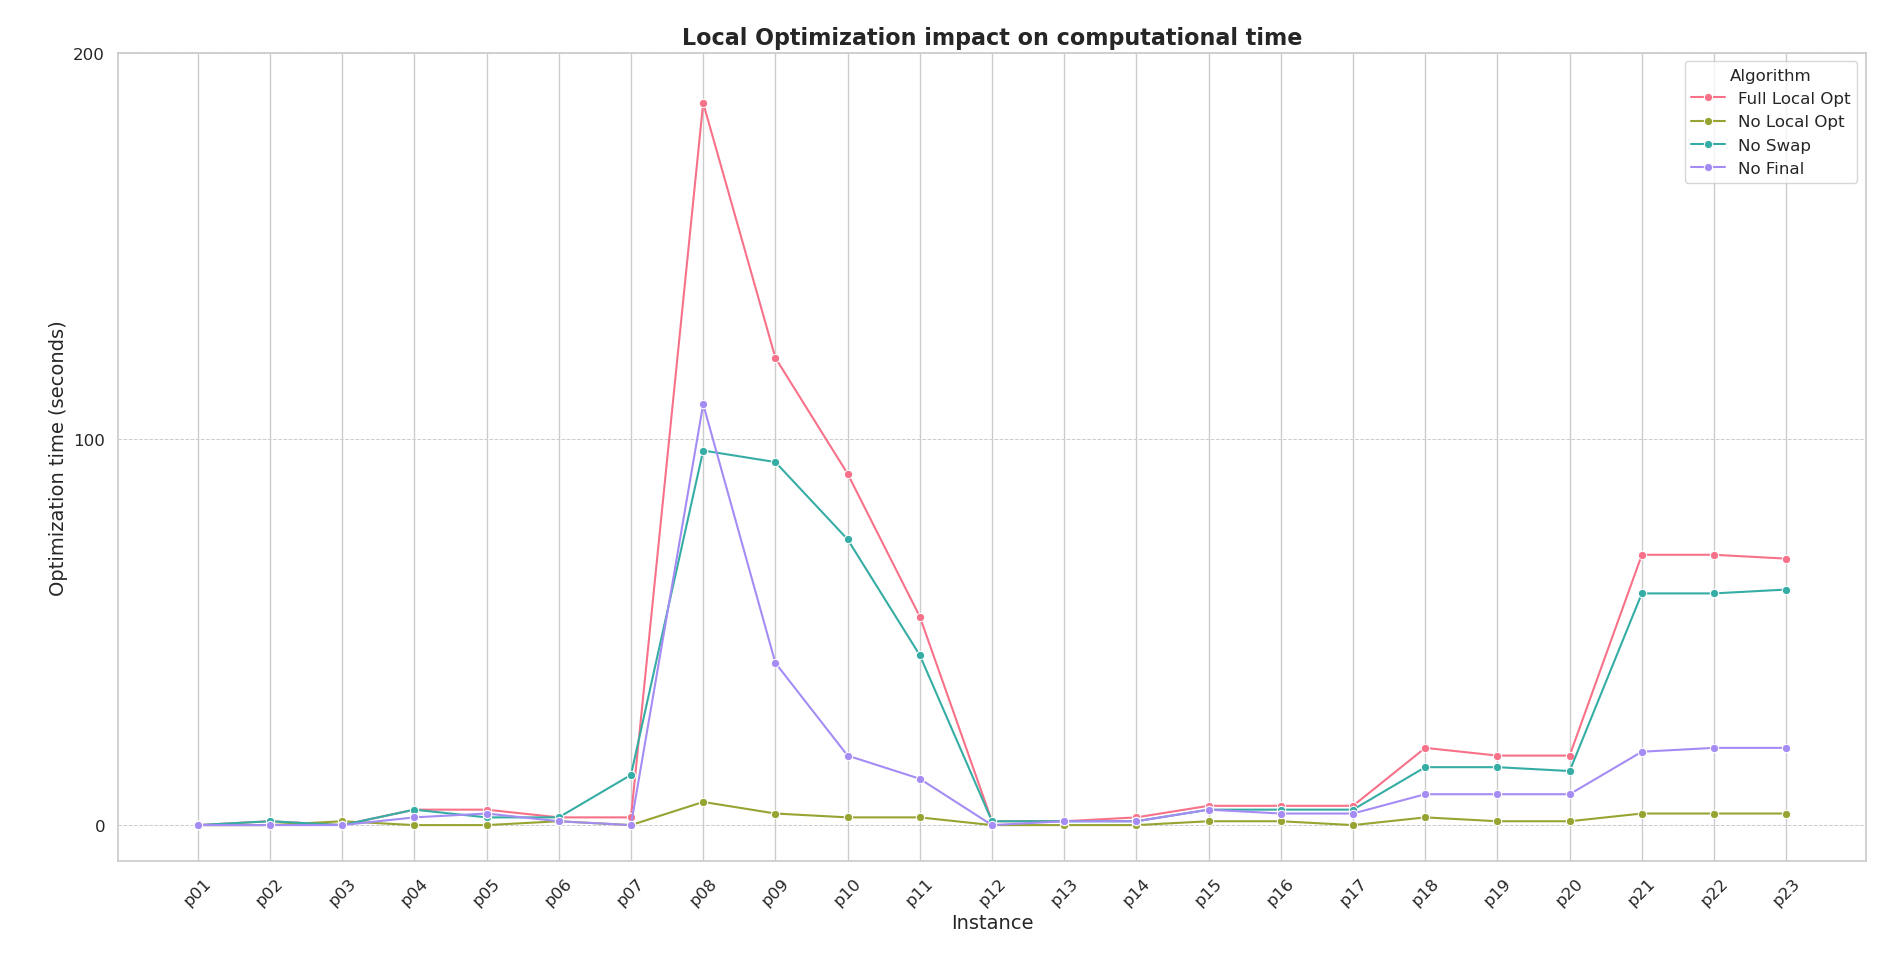
\includegraphics[width=\textwidth]{optimization_times_kmeans}
	\end{figure*}

	
	
	
	\clearpage
	\subsection{AACONC+ Results and Comparison to heuristics}
	% Please add the following required packages to your document preamble:
% \usepackage{booktabs}
% \usepackage{graphicx}
\begin{table*}[!ht]
	\begin{minipage}{\columnwidth}
		\centering
		\caption{AACONC+ Results}
	\resizebox{\textwidth}{!}{%
		\begin{tabular}{@{}ccccccc@{}}
			\toprule
			\textbf{Instance} & \textbf{Best} & \textbf{Average} & \textbf{gap(\%)} & \textbf{Worst} & \textbf{gap(\%)} & \textbf{Average time(s)} \\
			\midrule
			p01-C & 178.56 & 196.74 & 10.18 & 225.60 & 26.34 & 141 \\
			\midrule
			p02-C & 172.73 & 196.57 & 13.8 & 234.78 & 35.92 & 123 \\
			\midrule
			p03-C & 173.82 & 187.26 & 7.73 & 210.15 & 20.90 & 305 \\
			\midrule
			p04-C & 629.88 & 644.84 & 2.37 & 675.63 & 7.26 & 1203 \\
			\midrule
			p05-C & 573.03 & 613.47 & 7.06 & 692.44 & 20.84 & 884 \\
			\midrule
			p06-C & 379.10 & 390.34 & 2.96 & 403.39 & 6.41 & 1316 \\
			\midrule
			p07-C & 288.24 & 297.91 & 3.35 & 314.78 & 9.21 & 798 \\
			\midrule
			p08-C & 3023.77 & 3100.23 & 2.53 & 3265.97 & 8.01 & 1635 \\
			\midrule
			p09-C & 1705.03 & 1774.86 & 4.10 & 1846.92 & 8.32 & 3391 \\
			\midrule
			p10-C & 1286.28 & 1319.78 & 2.60 & 1349.47 & 4.91 & 3549 \\
			\midrule
			p11-C & 992.16 & 1035.63 & 4.38 & 1061.7 & 7.01 & 3600 \\
			\midrule
			p12-C & 1082.12 & 1123.30 & 3.81 & 1175.39 & 8.62 & 446 \\
			\midrule
			p13-C & 1099.02 & 1135.30 & 3.30 & 1191.96 & 8.46 & 491 \\
			\midrule
			p14-C & 1111.12 & 1123.33 & 1.10 & 1170.17 & 5.31 & 423 \\
			\midrule
			p15-C & 1166.08 & 1202.57 & 3.13 & 1228.27 & 5.33 & 2471 \\
			\midrule
			p16-C & 1178.51 & 1209.60 & 2.64 & 1241.67 & 5.36 & 2146 \\
			\midrule
			p17-C & 1142.74 & 1199.88 & 5.00 & 1253.47 & 9.69 & 2628 \\
			\midrule
			p18-C & 1231.96 & 1263.90 & 2.59 & 1296.42 & 5.23 & 3368 \\
			\midrule
			p19-C & 1250.26 & 1266.54 & 1.30 & 1284.23 & 2.72 & 3600 \\
			\midrule
			p20-C & 1246.36 & 1266.70 & 1.63 & 1280.77 & 2.76 & 3445 \\
			\midrule
			p21-C & 1296.19 & 1330.11 & 2.62 & 1347.09 & 3.93 & 3600 \\
			\midrule
			p22-C & 1317.94 & 1332.07 & 1.07 & 1354.61 & 2.78 & 3600 \\
			\midrule
			p23-C & 1319.93 & 1341.50 & 1.63 & 1356.62 & 2.78 & 3600 \\
			\midrule
			\textbf{Average} & 1037.52 & 1067.59 & 3.46 & 1107.25 & 8.68 & 2021.13 \\ \bottomrule
		\end{tabular}%
	}
	\label{tab:table2}
\end{minipage}
\end{table*}\;
	% Please add the following required packages to your document preamble:
% \usepackage{booktabs}
% \usepackage{graphicx}
% \usepackage{amsmath}
\begin{table*}[h!]
	\begin{minipage}{0.7\columnwidth}
		\centering
		\caption{AACONC+ best and heuristic results}
		\resizebox{\textwidth}{!}{%
			\begin{tabular}{@{}cccccc@{}}
				\toprule
				\textbf{Instance} & \textbf{AACONC+} & \textbf{heuristic (prox.)} & \textbf{gap(\%)} & \textbf{heuristic (k-means)} & \textbf{gap(\%)} \\
				\midrule
				p01-C & \textbf{178.56} & 217.42 & 21.76 & 191.03 & 6.98 \\
				\midrule
				p02-C & \textbf{172.73} & 219.2 & 26.90 & 188.60 & 9.19 \\
				\midrule
				p03-C & \textbf{173.82} & 214.84 & 23.60 & 185.82 & 6.90 \\
				\midrule
				p04-C & \textbf{629.88} & 668.81 & 6.18 & 694.96 & 10.33  \\
				\midrule
				p05-C & \textbf{573.03} & 630.78 & 10.08 & 624.33 & 8.95  \\
				\midrule
				p06-C & \textbf{379.10} & 435.42 & 14.86 & 416.25 & 9.80 \\
				\midrule
				p07-C & \textbf{288.24} & 309.48 & 7.37 & 314.41 & 9.08 \\
				\midrule
				p08-C & \textbf{3023.77} & 3333.93 & 10.26 & 3186.02 & 5.37  \\
				\midrule
				p09-C & \textbf{1705.03} & 1917.82 & 12.48 & 1964.49 & 15.22 \\
				\midrule
				p10-C & \textbf{1286.28} & 1493.13 & 16.08 & 1500.38 & 16.64  \\
				\midrule
				p11-C & \textbf{992.16} & 1145.75 & 15.48 & 1031.09 & 3.92  \\
				\midrule
				p12-C & \textbf{1082.12} & 1273.77 & 17.71 & 1273.77 & 17.71 \\
				\midrule
				p13-C & \textbf{1099.02} & 1226.63 & 11.61 & 1226.63 & 11.61  \\
				\midrule
				p14-C & \textbf{1111.12} & 1284.73 & 15.62 & 1284.73 & 15.62  \\
				\midrule
				p15-C & \textbf{1166.08} & 1347.67 & 15.57 & 1295.23 & 11.08 \\
				\midrule
				p16-C & \textbf{1178.51} & 1289.29 & 9.40 & 1289.29 & 9.40 \\
				\midrule
				p17-C & \textbf{1142.74} & 1320.91 & 15.59 & 1273.39 & 11.43  \\
				\midrule
				p18-C & 1231.96 & 1260.24 & 2.30 & \textbf{1211.56} & -1.66  \\
				\midrule
				p19-C & 1250.26 & 1266.92 & 1.33 & \textbf{1248.93} & -0.11  \\
				\midrule
				p20-C & 1246.36 & 1323.10 & 6.16 & \textbf{1234.12} & -0.98  \\
				\midrule
				p21-C & 1296.19 & 1363.18 & 5.17 & \textbf{1231.23} & -5.01  \\
				\midrule
				p22-C & 1317.94 & 1295.67 & -1.69 & \textbf{1230.99} & -6.60  \\
				\midrule
				p23-C & 1319.93 & 1252.36 & -5.12 & \textbf{1222.63} & -7.37 \\
				\midrule
				\textbf{Average} & \textbf{1037.52} & 1134.39 & 11.24 & 1100.86 & 6.84 \\ \bottomrule
			\end{tabular}%
		}
	\end{minipage}
\end{table*}
\;
	\captionsetup{justification=centering}  % Center the captions
	\begin{figure*}[h!]
		\centering
		\caption{Comparison to the best solution found by AACONC+}
		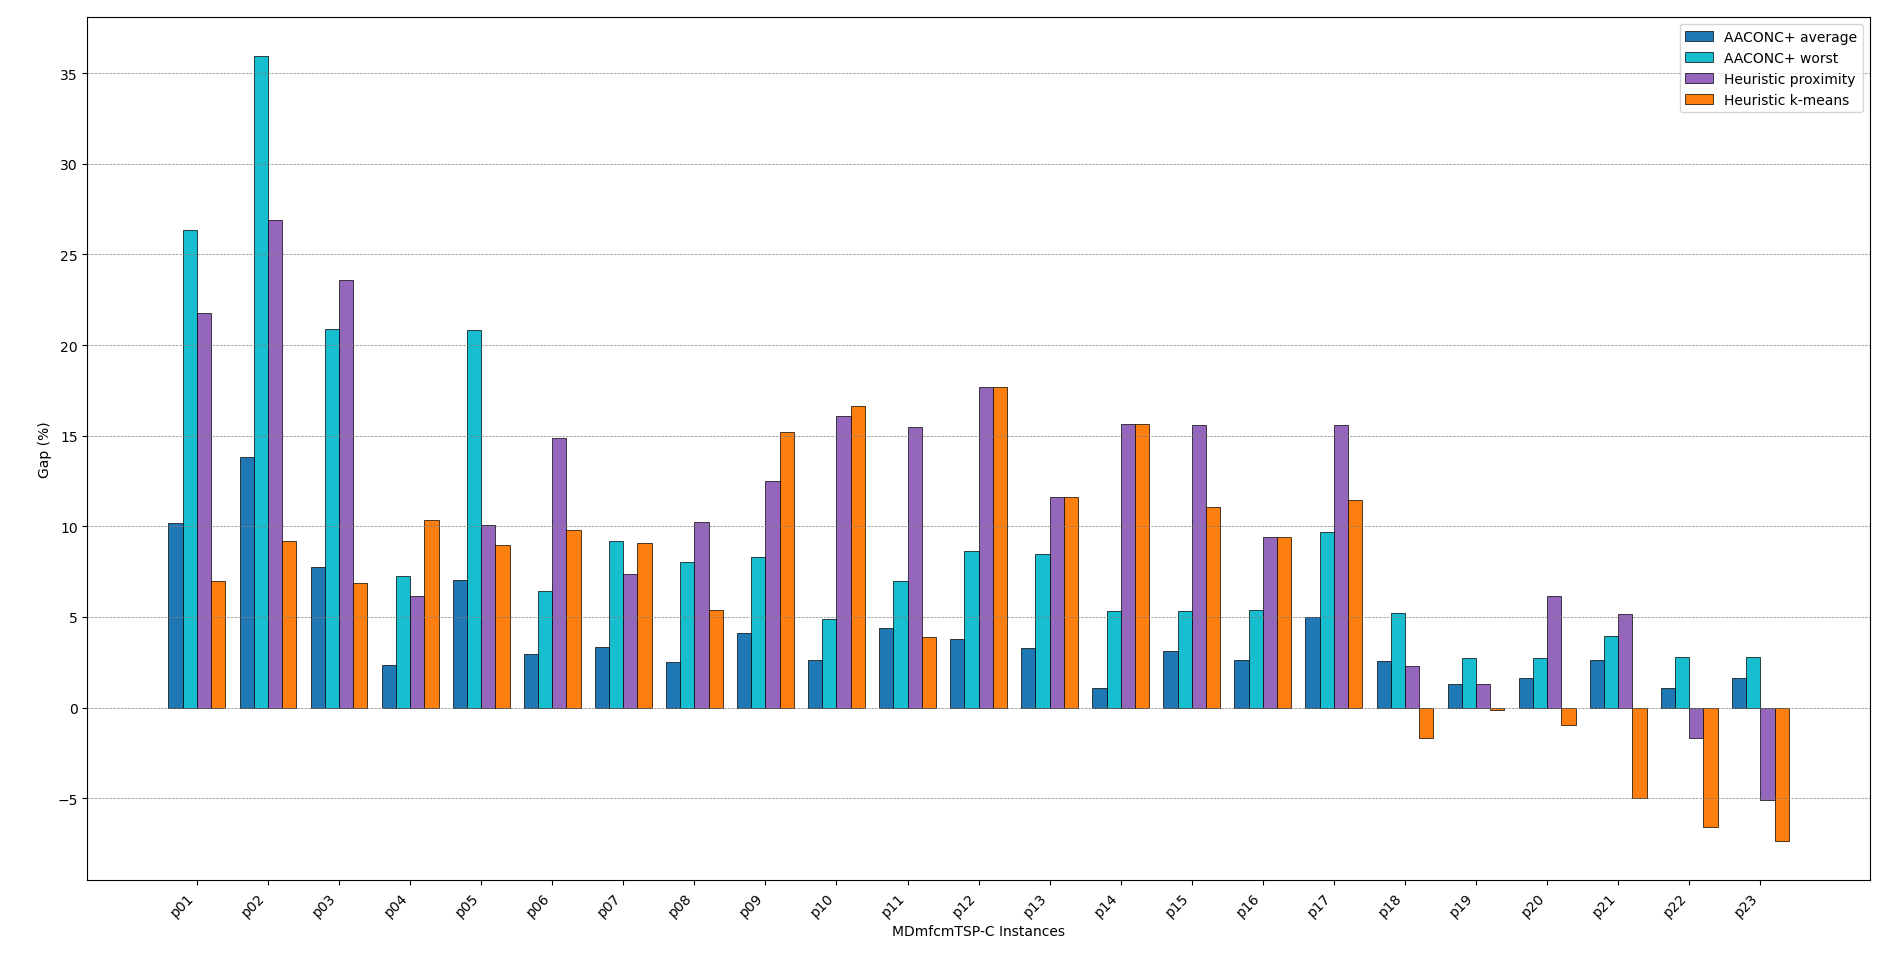
\includegraphics[width=\textwidth]{gaps_to_aco_best}
	\end{figure*}
	\begin{figure*}[h!]
		\centering
		\caption{Comparison of best results found}
		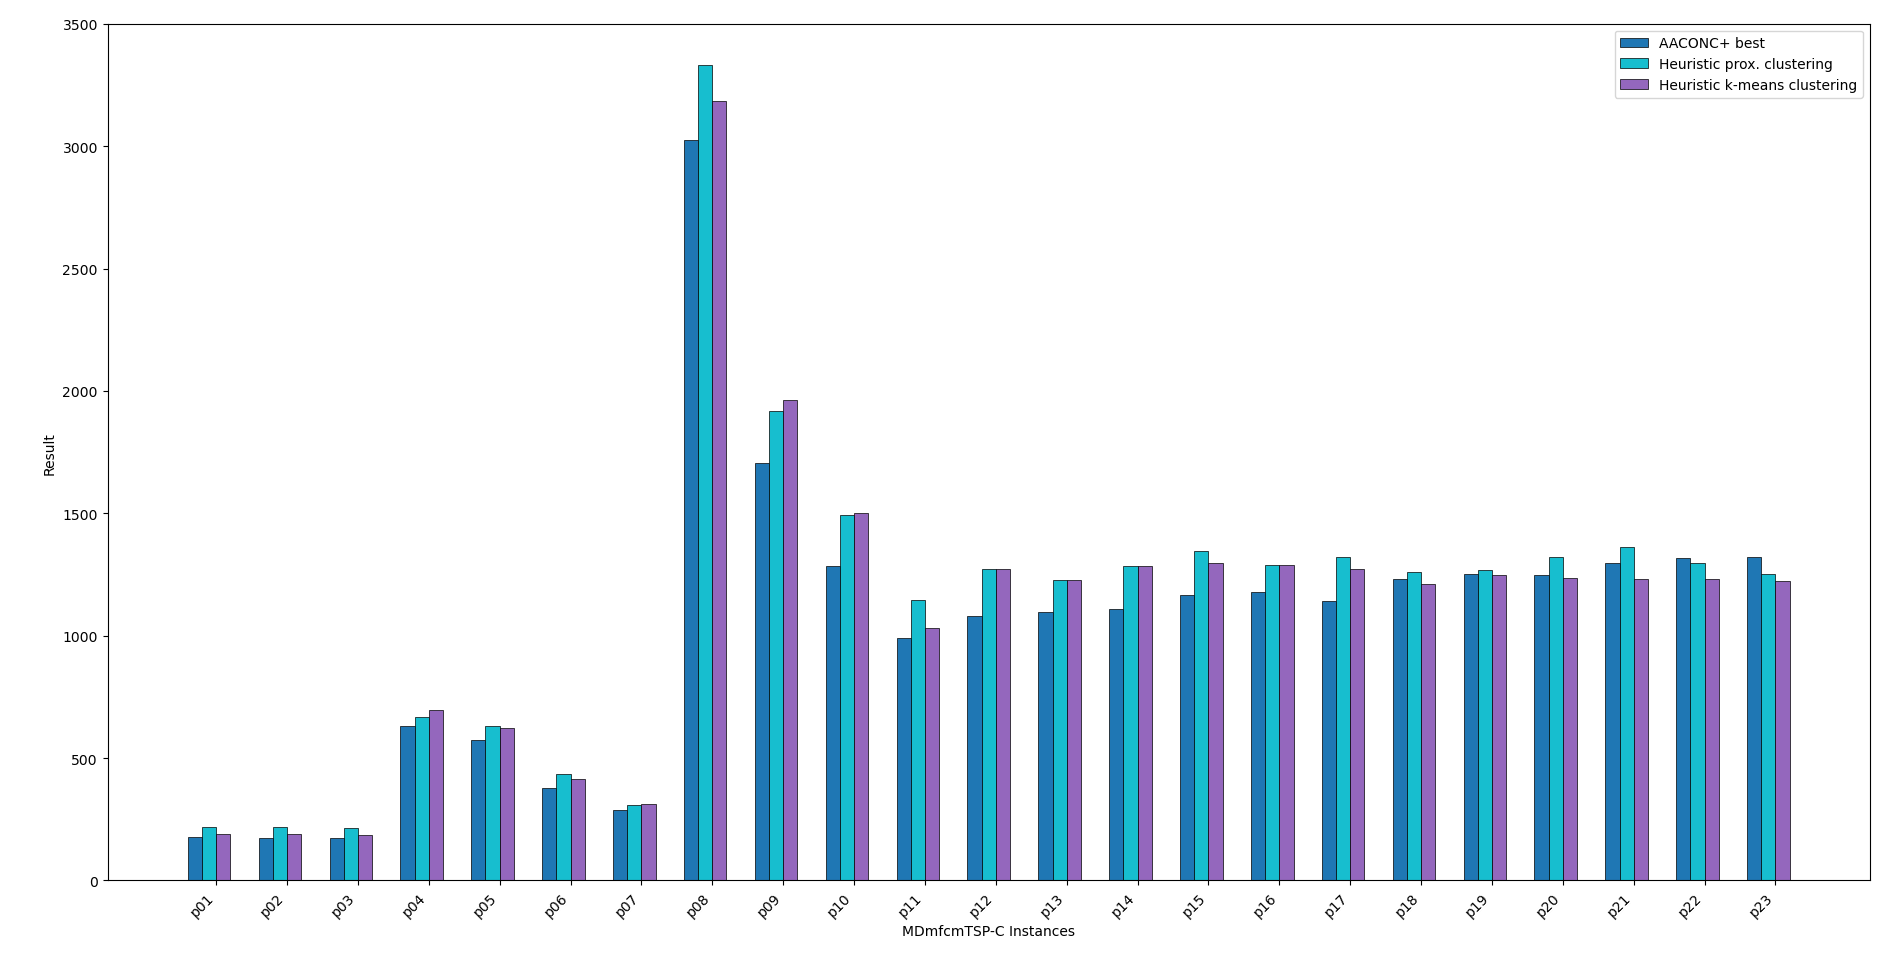
\includegraphics[width=\textwidth]{best_results_comp_barGraph}
	\end{figure*}

	\begin{figure*}[h!]
		\centering
		\caption{Comparison to the best solution found by AACONC+}
		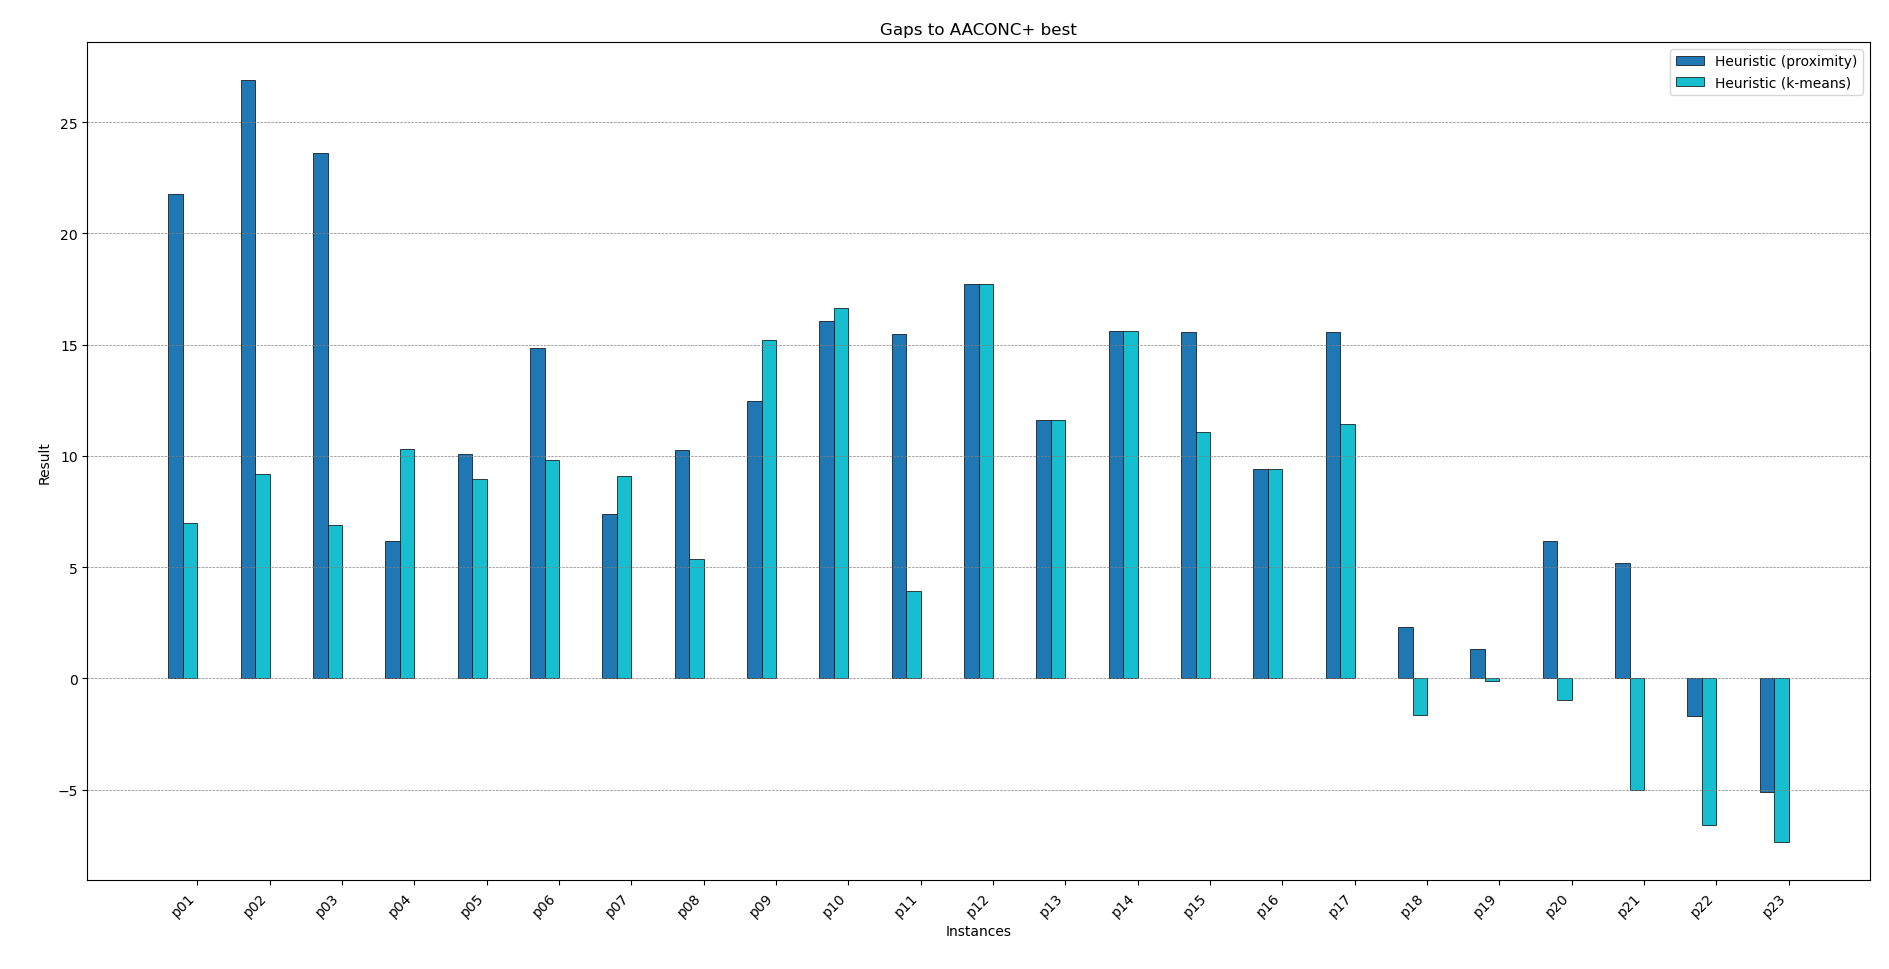
\includegraphics[width=\textwidth]{heuristics_comp_to_best_gaps}
	\end{figure*}
	\begin{figure*}[h!]
		\centering
		\caption{Comparison to the average solution found by AACONC+}
		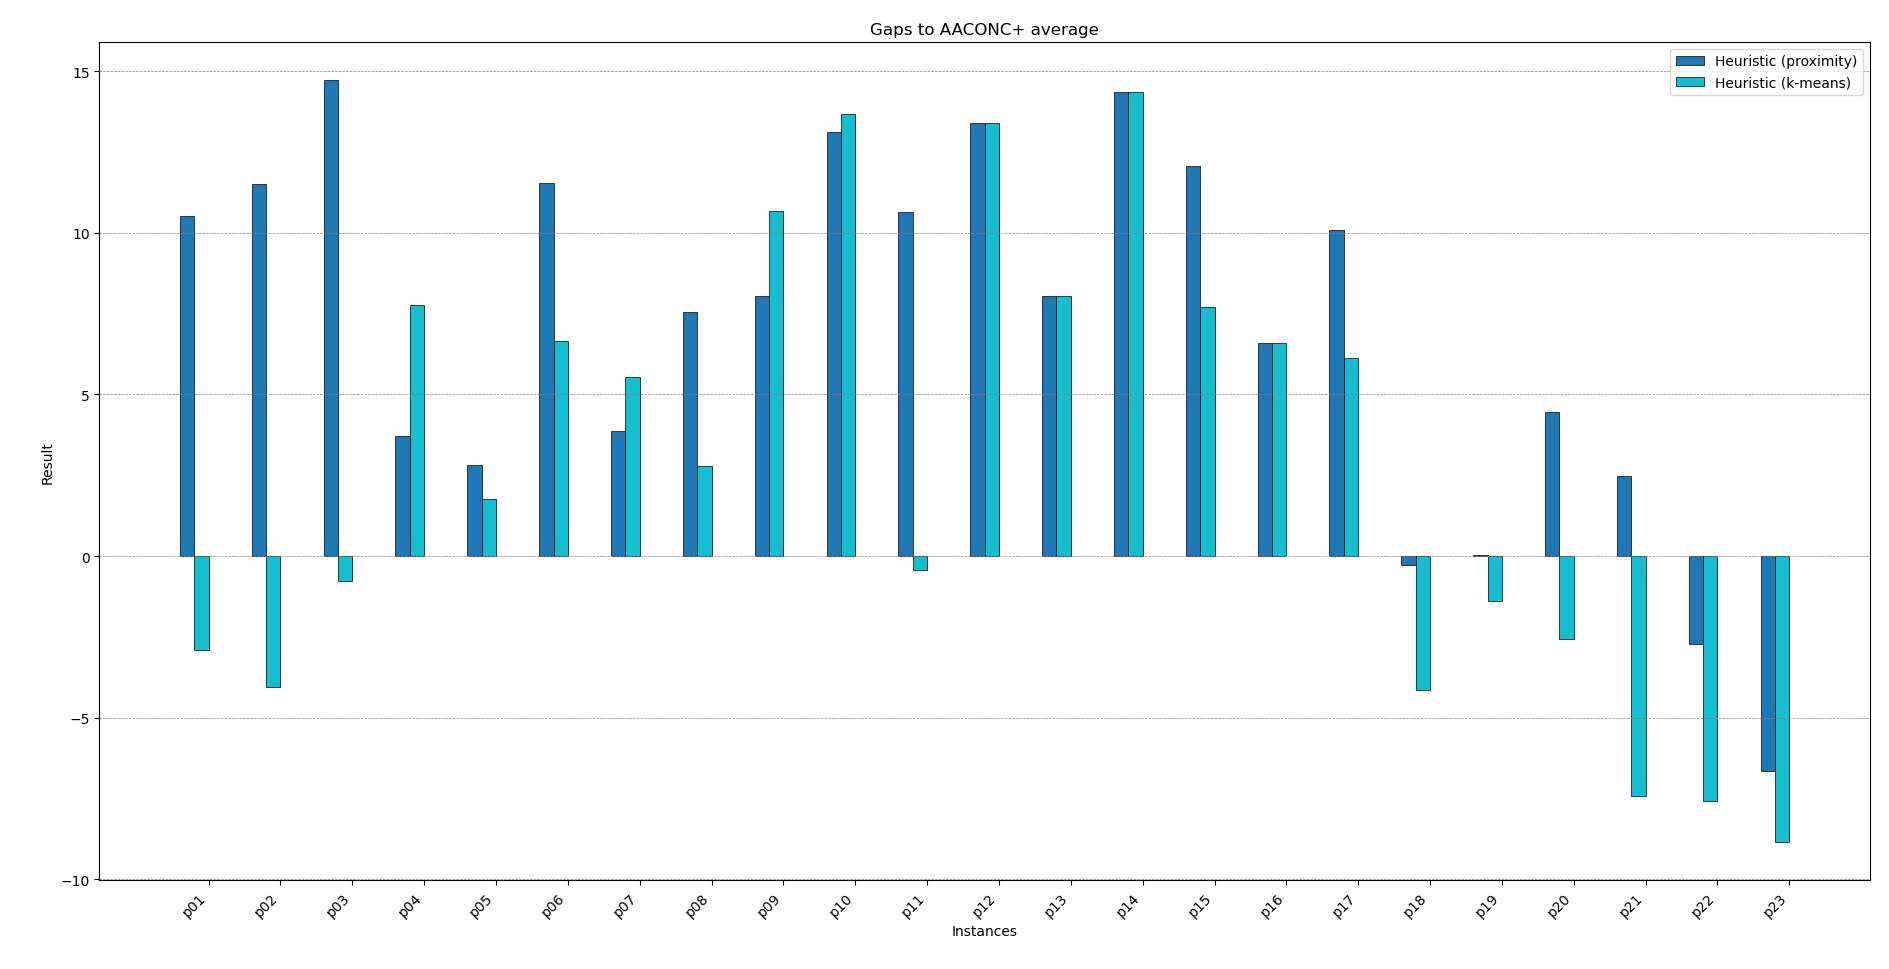
\includegraphics[width=\textwidth]{heuristics_comp_to_avg_gaps}
	\end{figure*}
	\begin{figure*}[h!]
		\centering
		\caption{Comparison to the worst solution found by AACONC+}
		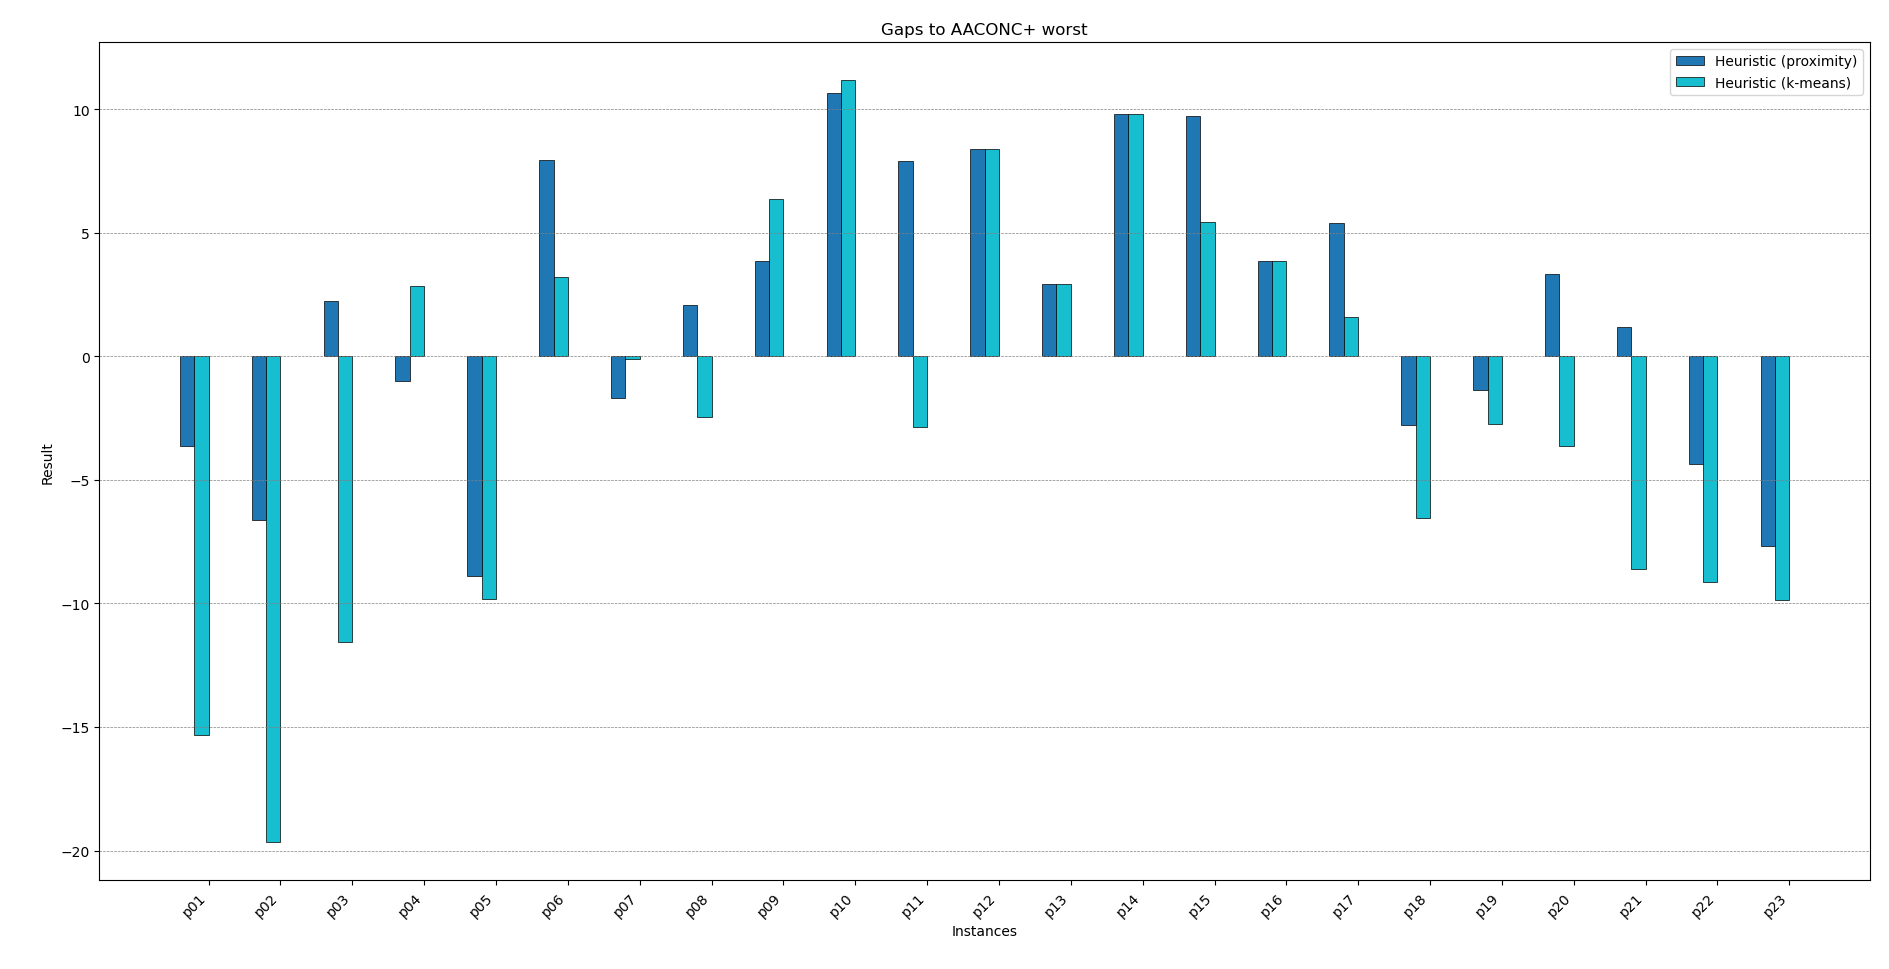
\includegraphics[width=\textwidth]{heuristics_comp_to_worst_gaps}
	\end{figure*}
	\begin{figure*}[h!]
		\centering
		\caption{Comparison of best results found}
		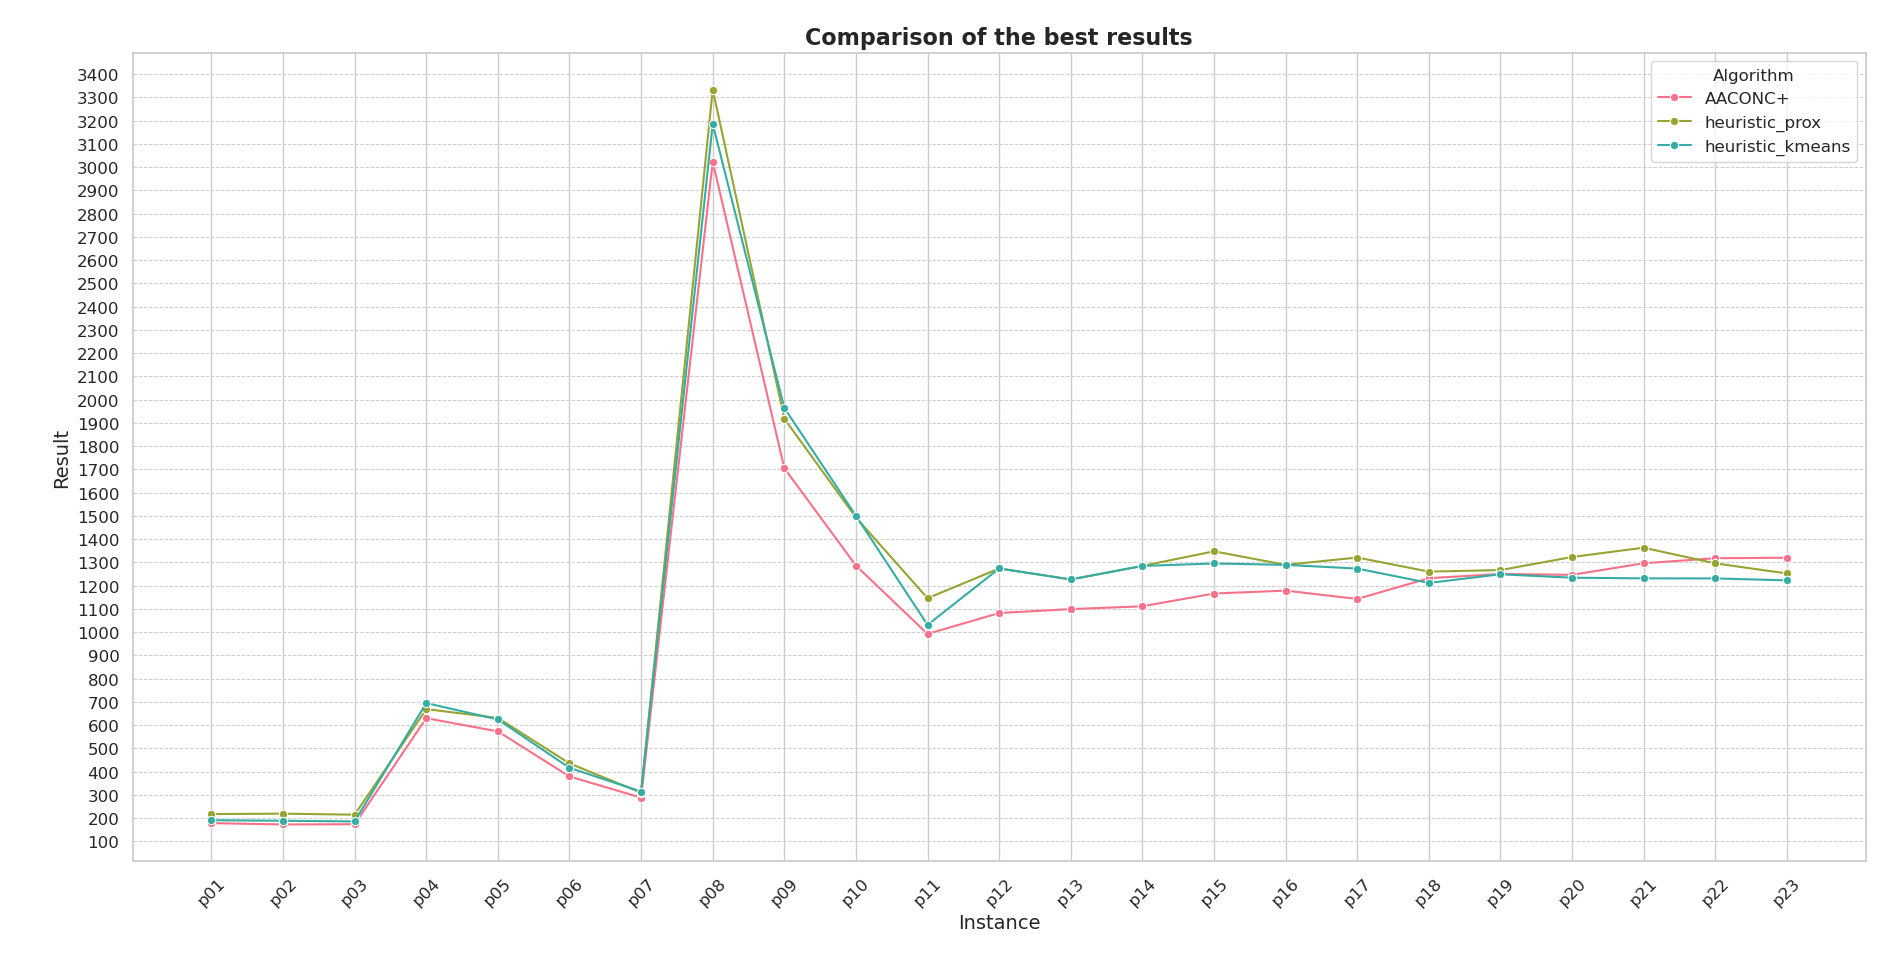
\includegraphics[width=\textwidth]{best_results_all_lineGraph}
	\end{figure*}
	\begin{figure*}[h!]
		\centering
		\caption{}
		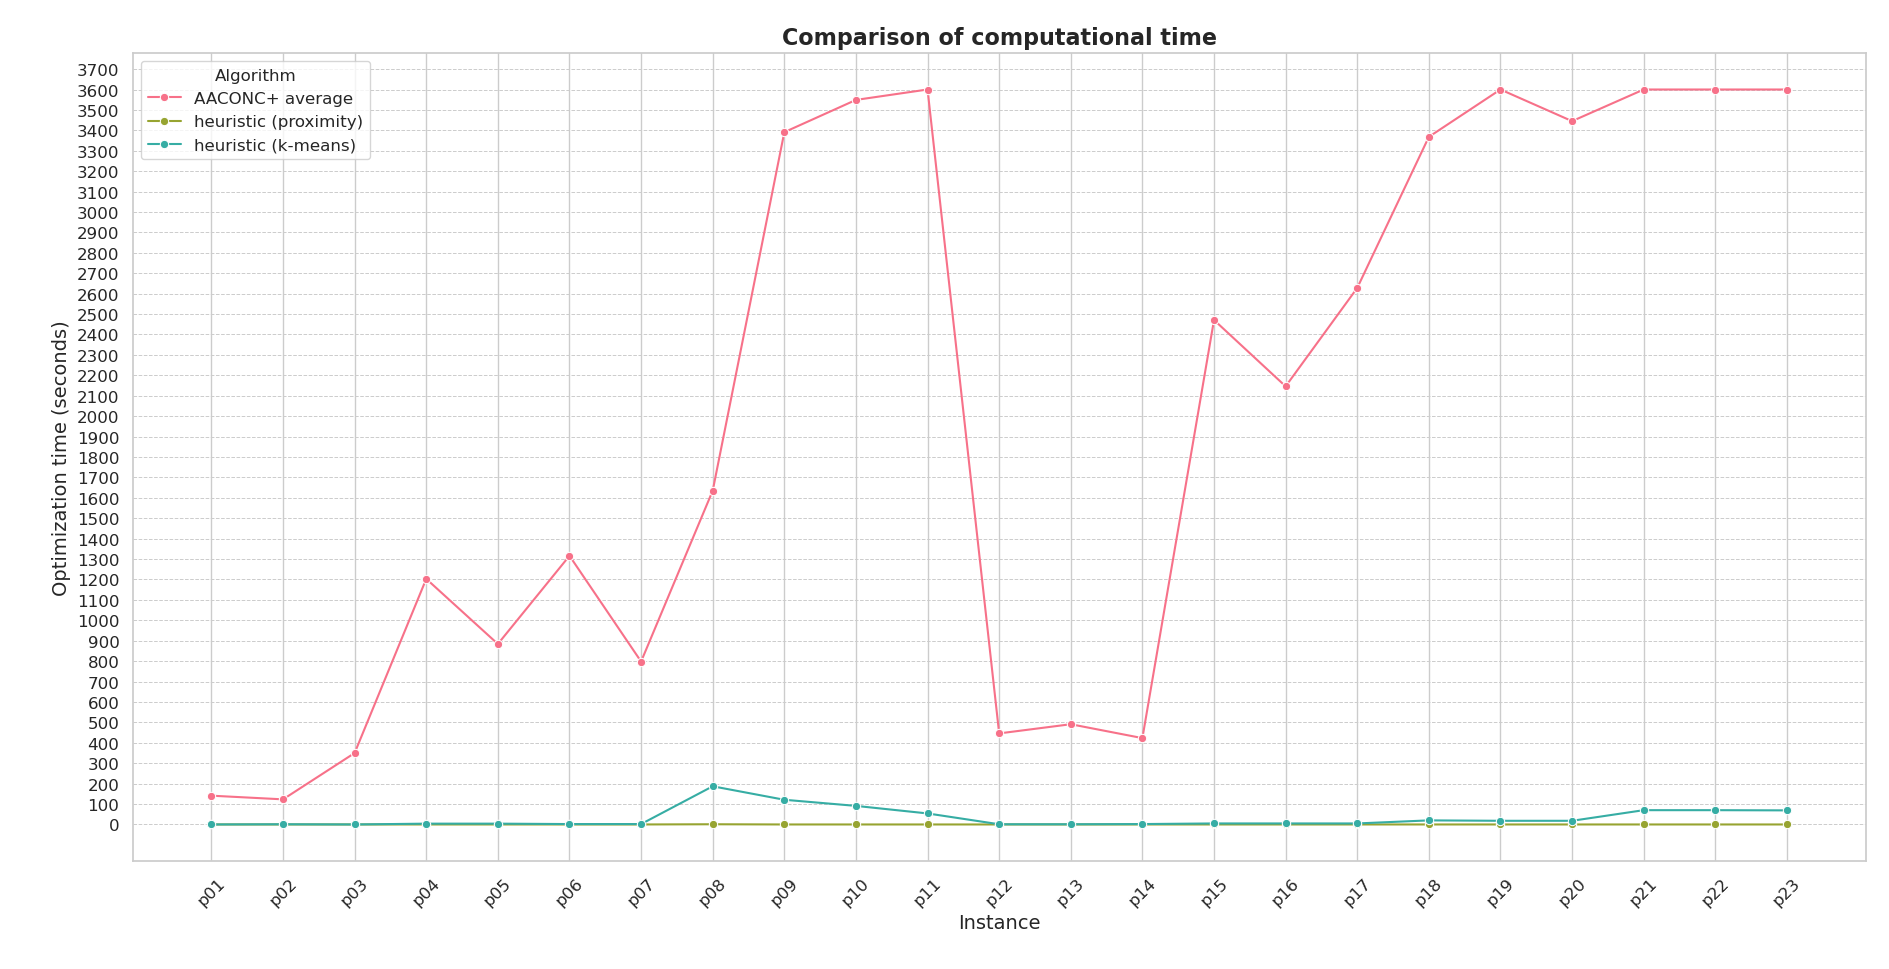
\includegraphics[width=\textwidth]{optimization_times}
	\end{figure*}
	
	
	
	\clearpage
	
	\twocolumn
	
	\section{Related Literature}
	% Please add the following required packages to your document preamble:
% \usepackage{booktabs}
% \usepackage{graphicx}
\begin{table*}[]
	\caption{Drone-related Routing literature}
	\resizebox{\textwidth}{!}{%
		\begin{tabular}{@{}lllcccl@{}}
			\toprule
			\textbf{Reference} & \textbf{Problem} & \textbf{Scale} & \textbf{Tandem} & \textbf{Flight endurance} & \textbf{Capacitated*} & \textbf{Solution Method} \\ \midrule
			Murray \& Chu (2015) & FSTSP & 1-Truck 1-Drone 1-Depot & Yes & Yes & No & MILP, Heuristics \\
			\midrule
			& PDSTSP & 1-Truck n-Drone 1-Depot & No & Yes & No & MILP, Heuristics \\
			\midrule
			Ha et al. (2015) & FSTSP & 1-Truck 1-Drone 1-Depot & Yes & Yes & No & MIP, Heuristics \\
			\midrule
			Freitas \& Penna (2018) & FSTSP & 1-Truck 1-Drone 1-Depot & Yes & Yes & No & IP, Heuristics \\
			\midrule
			Boccia et al. (2021) & FSTSP/PDSTSP & 1-Truck 1-Drone 1-Depot & Yes & Yes & No & MILP, Heuristics \\
			\midrule
			Dell'Amico et al. (2021) & FSTSP & 1-Truck 1-Drone 1-Depot & Yes & Yes & No & MILP \\
			\midrule
			Dell'Amico et al. (2021) & FSTSP & 1-Truck 1-Drone 1-Depot & Yes & Yes & No & Branch and bound, Heuristic  \\
			\midrule
			Kuroswiski et al. (2023) & FSTSP & 1-Truck 1-Drone 1-Depot & Yes & Yes & No & MILP, Metaheuristics \\
			\midrule
			Pilcher (2023) & FSTSP & 1-Truck 1-Drone 1-Depot & Yes & Yes & No & Self-adaptive GA \\
			\midrule
			Mbiadou Saleu et al. (2018) & PDSTSP & 1-Truck n-Drone 1-Depot & No & Yes & No & MILP, Heuristics \\
			\midrule
			Dinh et al. (2021) & PDSTSP & 1-Truck n-Drone 1-Depot & No & Yes & No & Metaheuristics \\
			\midrule
			Nguyen et al. (2022) & PDSTSP & 1-Truck n-Drone 1-Depot & No & Yes & No & MILP \\
			\midrule
			Mbiadou Saleu et al. (2022) & PDSMTSP & m-Truck n-Drone 1-Depot & No & Yes & No & MILP, Metaheuristics \\
			\midrule
			Montemanni et al. (2023) & PDSTSP & 1-Truck n-Drone 1-Depot & Yes & Yes & No & Constraint Programming  \\
			\midrule
			Nguyen et al. (2023) & PDSTSP-c & 1-Truck n-Drone 1-Depot & No & Yes & No & MILP, Metaheuristics  \\
			\midrule
			Montemanni et al. (2024) & PDSTSP-c & 1-Truck n-Drone 1-Depot & No & Yes & No & MILP, Constraint Programming \\
			\midrule
			Ham (2018) & PDSTSP$^{+DP}$ & m-Truck n-Drone 2-Depot & No & Yes & No & Constraint Programming \\
			\midrule
			Agatz et al. (2018) & TSP-D & 1-Truck 1-Drone 1-Depot & Yes & Yes & No & IP, Heuristics \\
			\midrule
			Yurek et al. (2018) & TSP-D & 1-Truck 1-Drone 1-Depot & Yes & Yes & No & MIP, Heuristics \\
			\midrule
			Ha et al. (2018) & min-cost TSP-D & 1-Truck 1-Drone 1-Depot & Yes & Yes & No & MILP, GRASP, TSP-LS \\
			\midrule
			Dorling et al. (2016) & DDPs & 0-Truck n-Drone 1-Depot & No & Yes & Yes & MILP, SA \\
			\midrule
			Ulmer \& Thomas (2018) & SDDPHF & m-Truck n-Drone 1-Depot & No & No & No & Adaptive dynamic programming \\
			\midrule
			Salama \& Srinivas (2020) & JOCR & 1-Truck n-Drone 1-Depot & Yes & Yes & No & IP, MILP, Heuristics \\
			\midrule
			Lu et al. (2022) & FDTSP & 1-Truck n-Drone 1-Depot & Yes & Yes & No & Heuristics, Metaheuristics \\
			\midrule
			Lan (2024) & TSPTWD & 1-Truck 1-Drone 1-Depot & Yes & Yes & No & Metaheuristics \\
			\midrule
			Wang et al. (2017) & VRPD & m-Truck n-Drone 1-Depot & Yes & Yes & Yes & Problem formulation, theoretical study \\
			\midrule
			Schermer et al. (2018) & VRPD & m-Truck n-Drone 1-Depot & Yes & Yes & Yes & Heuristics \\
			\midrule
			Sacramento et al. (2019) & VRP-D & m-Truck m-Drone 1-Depot & Yes & Yes & Yes* & MIP, ALNS \\
			\midrule
			Schermer et al. (2019) & VRPDERO & m-Truck n-Drone 1-Depot & No & Yes & No & MILP, VNS, TS \\
			\midrule
			Nguyen et al. (2022) & PDSVRP & m-Truck n-Drone 1-Depot & No & Yes & Yes & MILP, Metaheuristics \\
			\midrule
			Schermer et al. (2019) & VRPD & m-Truck n-Drone 1-Depot & Yes & Yes & No & MILP, Matheuristic \\
			\midrule
			Wang \& Sheu (2019) & VRPD & m-Truck n-Drone 1-Depot & No & Yes & Yes & MIP, branch-and-price \\
			\midrule
			Euchi \& Sadok (2021) & VRP-D & m-Truck m-Drone 1-Depot & Yes & Yes & Yes & MILP, HGA \\
			\midrule
			Lei et al. (2022) & VRPD & m-Truck m-Drone 1-Depot & Yes & Yes & Yes & Dynamical Artificial Bee Colony \\
			\midrule
			Karak et al. (2019) & HVDRP & m-Truck n-Drone 1-Depot & Yes & Yes & Yes(Drones) & MIP, Heuristics \\
			\midrule
			Kuo et al. (2022) & VRPDTW & m-Truck m-Drone 1-Depot & Yes & Yes & Yes & MIP, VNS \\
			\midrule
			Stodola et al. (2024) & MDVRP-D & m-Truck m-Drone m-Depot & Yes & Yes & Yes & ACO \\
			\midrule
			Oikonomou et al. (2019) & mfcmTSP & 1-Truck 1-Drone 1-Depot & No & No & No & Heuristics \\
			\midrule
			This paper & MD-mfcmTSP & m-Truck n-Drone k-Depot & No & No & Yes & Metaheuristics, Heuristics \\
			\bottomrule
		\end{tabular}%
	}
\end{table*}
	At the same time, it is important that we address flight range limitations. Such limitations have important roles in much of
	the existing drone routing research. However, even he first drones developed by Amazon and JD.com ahad a flight range of 15
	to 20 miles [33, 56]. Such a range is suitable to allow out and back travel in the medium-sized cities in which the authors live,
	Braunschweig, Germany, and Iowa City, United States. In fact, it is suitable for many larger cities such as Hamburg, Munich,
	and Paris. Thus, in contrast to other drone applications, in this work, we do not consider flight range as a limiting factor (Ulmer \& Thomas (2018)).
	
	
	
\end{document}